\documentclass[a4paper,10pt]{article}

\usepackage[utf8]{inputenc}
\usepackage[T1]{fontenc}
\usepackage[english]{babel}

\usepackage{color}
\usepackage{float}
\usepackage{fancyvrb}

\usepackage{amssymb}
\usepackage{amsmath}

\usepackage{listings}
\usepackage{comment}
\usepackage[boxed]{algorithm2e}
\usepackage{graphicx}
\usepackage{subcaption}
\usepackage{subfig}
\usepackage{natbib}

\usepackage{amsthm}
\theoremstyle{plain}

\theoremstyle{definition}
\newtheorem{defn}{Definition}
% \begin{defn}Here is a new definition.\end{defn}

\DeclareGraphicsExtensions{.png}

\definecolor{dkgreen}{rgb}{0,0.45,0}
\definecolor{gray}{rgb}{0.5,0.5,0.5}
\definecolor{mauve}{rgb}{0.30,0,0.30}

\lstset{frame=tb,
  language=Java,
  aboveskip=3mm,
  belowskip=3mm,
  showstringspaces=false,
  columns=flexible,
  basicstyle={\small\ttfamily},
  numbers=left,
  numberstyle=\footnotesize,
  keywordstyle=\color{dkgreen}\bfseries,
  commentstyle=\color{red},
  stringstyle=\color{mauve},
  frame=single,
  breaklines=true,
  breakatwhitespace=false
  tabsize=1
}

\title{ Parameterless clustering by dynamic tree-cutting \rule{10cm}{0.5mm}}
\author{Simon Lehmann Knudsen \\
	simkn15@student.sdu.dk \\
	ECTS: 10 \\
	04/09-2017 - 31/01-2018 \\
	5th semester in Computer Science \\
	Supervisor: Richard Röttger
\\\rule{5.5cm}{0.5mm}\\}
\date{31/01-2018}

\begin{document}
\maketitle

\newpage
\tableofcontents

%%%%%%%%%%%%%%%%%%%%%%%%%%%%%%%%%%%%%%%%%%%%%%%%%%
%%%%%%%%%%%%%%%%%%%%%%%%%%%%%%%%%%%%%%%%%%%%%%%%%%
%%%%%%%%%%%%%%%%%%%%%%%%%%%%%%%%%%%%%%%%%%%%%%%%%%
\newpage
\section*{Abstract}
%%%%%%%%%%%%%%%%%%%%%%%%%%%%%%%%%%%%%%%%%%%%%%%%%%
%%%%%%%%%%%%%%%%%%%%%%%%%%%%%%%%%%%%%%%%%%%%%%%%%%
%%%%%%%%%%%%%%%%%%%%%%%%%%%%%%%%%%%%%%%%%%%%%%%%%%

%%%%%%%%%%%%%%%%%%%%%%%%%%%%%%%%%%%%%%%%%%%%%%%%%%
%%%%%%%%%%%%%%%%%%%%%%%%%%%%%%%%%%%%%%%%%%%%%%%%%%
\subsection*{Background}
%%%%%%%%%%%%%%%%%%%%%%%%%%%%%%%%%%%%%%%%%%%%%%%%%%
%%%%%%%%%%%%%%%%%%%%%%%%%%%%%%%%%%%%%%%%%%%%%%%%%%
Clustering describes the unsupervised learning task of grouping similar objects into so-called clusters. A cluster is a group of objects that are more similar to each other than those of another cluster. Clustering is used is applied in many different fields such as economics, marketing, astronomy and bioinformatics. The conclusion of the study from \cite{powerLimits} was that state-of-the-art clustering tools have limitations capturing the diversity of protein families and requires a specific parameter for every dataset which cannot be easily provided in practice. A cluster analysis consists of 5 steps according to Jain et al. \cite{19overview}. (*) Data Abstraction, (1) Preprocessing, (2) Proximity Calculation, (3) Clustering, (4) Evaluation. We want to investigate parameterless clustering by dynamic tree-cutting. We will extend Transitivity Clustering(TC) into Hierarchical Clustering(HC), which we call Transitivity-Hierarchical Clustering(THC). The used dataset is the Brown dataset \cite{brown}. Hierarchical Clustering produces a tree like structure - a dendrogram. Each node represents a cluster. For each node in the dendrogram we randomize the same data from the node, and look at the difference in cost of the actual data and the random data. This should give an indication of where to cut the branches in the dendrogram. The resulting tree is cut on different levels, and is the optimal clustering. 

%%%%%%%%%%%%%%%%%%%%%%%%%%%%%%%%%%%%%%%%%%%%%%%%%%
%%%%%%%%%%%%%%%%%%%%%%%%%%%%%%%%%%%%%%%%%%%%%%%%%%
\subsection*{Results}
%%%%%%%%%%%%%%%%%%%%%%%%%%%%%%%%%%%%%%%%%%%%%%%%%%
%%%%%%%%%%%%%%%%%%%%%%%%%%%%%%%%%%%%%%%%%%%%%%%%%%
To measure the quality of a clustering F-measure was implemented and yielding close to the same results as \cite{clustEval} for the small dataset, a subset of the Brown dataset. The returning dendrogram of THC was compared to the standard implementation of HC in R, and determined as feasible as we can find similarities. A total of 4 randomization approaches was tested. Approach 3 and 4 was found feasible to find the difference of costs in the dendrograms of the THC. Tests was made according find the difference of costs to find the proper cuts. Due to the scope of the project the findings have not been analyzed.

%%%%%%%%%%%%%%%%%%%%%%%%%%%%%%%%%%%%%%%%%%%%%%%%%%
%%%%%%%%%%%%%%%%%%%%%%%%%%%%%%%%%%%%%%%%%%%%%%%%%%
\subsection*{Conclusion}
%%%%%%%%%%%%%%%%%%%%%%%%%%%%%%%%%%%%%%%%%%%%%%%%%%
%%%%%%%%%%%%%%%%%%%%%%%%%%%%%%%%%%%%%%%%%%%%%%%%%%
The first steps of finding a pattern or indications of the proper cuts in a dendrogram have been made. F-measure was implemented such that we can measure the quality of a clustering. TC was successfully extended into a HC approach. Two randomization approaches looks feasible at this point. Several tests have been made on measures the difference of costs in a dendrogram for each node of the actual data and the random data. Although the plots have not been fully analyzed they do seem promising. At this point we do not have clear knowledge of this approach is feasible or infeasible. To answer this we need to take the following steps: (1) Analyze the produced information, (2) Alter THC such that it can cut the dendrogram on different branches and return a clustering result, (3) Measure the result with F-measure against the gold standard, (4) Repeatedly analyze produced data and try different ways to find the cuts, until we can deem this approach for parameterless clustering by dynamic tree-cutting feasible or infeasible.

%%%%%%%%%%%%%%%%%%%%%%%%%%%%%%%%%%%%%%%%%%%%%%%%%%
%%%%%%%%%%%%%%%%%%%%%%%%%%%%%%%%%%%%%%%%%%%%%%%%%%
%%%%%%%%%%%%%%%%%%%%%%%%%%%%%%%%%%%%%%%%%%%%%%%%%%
\newpage
\section{Introduction}
%%%%%%%%%%%%%%%%%%%%%%%%%%%%%%%%%%%%%%%%%%%%%%%%%%
%%%%%%%%%%%%%%%%%%%%%%%%%%%%%%%%%%%%%%%%%%%%%%%%%%
%%%%%%%%%%%%%%%%%%%%%%%%%%%%%%%%%%%%%%%%%%%%%%%%%%
Clustering describes the unsupervised learning task of grouping similar objects together into so-called clusters. Due to the versatility, clustering is applied in almost all scientific fields, like economics, marketing, astronomy and many others \cite{clusteringOverview}. In the field of bioinformatics, cluster analyses are used, e.g. analysis of microarray, cancer subtyping, protein homology detection, and many more \cite{clusteringOverview}. The application fields are very different, but the researcher faces similar decisions and challenges \cite{clusteringOverview}.
A cluster is a group of objects that are more similar to each other than those of another cluster. Although this definition is clear, it becomes more vague when recognizing clusters in the plane. Figure \ref{fig:clusterShapes} shows three different cluster shapes. One of the major problems of clustering is the absence of a clear definition of a \textit{good} clustering \cite{clusteringOverview}.
\begin{figure}
	\centering
	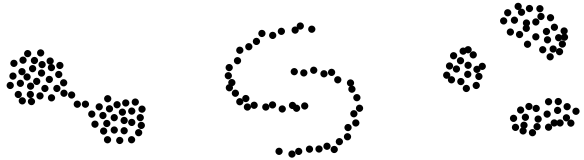
\includegraphics[scale=0.4]{./pictures/clusterShapes.png}
	\caption{Examples of cluster shapes}
	\label{fig:clusterShapes}
\end{figure}
Given a set of N objects $X = \{ x_1, \dots, x_N \}$, the following types of clustering tasks can be differentiated \cite{15overview}:
\begin{itemize}
	\item Partitional Clustering: The task of seeking a k-partition $C = \{ C_1, \dots, C_k \}$ of X, such that:
	\begin{enumerate}
		\item $C_i \neq \emptyset, i = 1, \dots, k$
		\item $\cup_{C_i \in C} C_i = X$
		\item $C_i \cap C_j = \emptyset \quad i,j = 1, \dots, k, i \neq j$
	\end{enumerate} 
	\item Overlapping Clustering: Follows the same principle as the partitional clustering with the difference that condition 3 does not hold. Each object can be a member of several clusters.
	\item Fuzzy Clustering: Assigns each object $x_i$ a degree of membership $u_{i,j}$ to each cluster $C_j$ of the k partitioning $C = \{ C_1, \dots, C_k \}$, such that
	\begin{enumerate}
		\item $\sum_{i = 1}^{k} u_{i,j} = 1 \quad \forall i$
		\item $0 < \sum_{i = 1}^{k} u_{i.j} < N \quad \forall i$
	\end{enumerate}
	\item Hierarchical Clustering: The task of constructing a tree-like nested structure of partitions of X. Further discussion and definitions will be derived in Section \ref{sec:hierarhicalClustering}.
\end{itemize}
The above definition only state what technically can be considered a clustering. They do not claim any requirements for a \textit{good} or \textit{bad} clustering. Putting all objects into one cluster, or setting all objects as their own cluster does not yield any insights. Judging the quality of a clustering is a non-trivial task, and is highly dependent on the situation. There exist no universally agreed-upon definition of the term cluster, due to the subjectivity of clustering \cite{15overview}. Finding the proper clustering method requires a deep knowledge of the different clustering tools, as well as the domain of the dataset. The determination of the best cluster criteria can be regarded as one of the most challenging questions when performing a cluster analysis \cite{clusteringOverview}. There exist no overall best-performer clustering tool, not even when limited to the same dataset type. The quality of the result if always highly dependent on the actual dataset \cite{17overview}. When sorting \textit{n} objects into \textit{m} clusters, this totals to 
\begin{equation*}
\frac{1}{m!}\sum_{k = 0}^{k - m} (-1)^{m - k}  { m \choose k } k^n
\end{equation*}
different possibilities. For 25 objects and 5 clusters the number of possibilities grows to $2.4 \cdot 10^{15}$ \cite{18overview}. The number of possibilities makes it absolutely infeasible to test all possible combinations to find the best clustering. 

With todays technologies we are producing a vast amount of genomic data at an ever increasing pace \cite{natureReviewsGenetics}. For us to gain any benefits from the data, it not only has to be analyzed, but in an efficient and automated manner \cite{powerLimits}. Even though there exists databases which provide information on protein family classification, e.g. SCOP$^2$ \cite{6powerLimits}, the number of protein families are growing \cite{7powerLimits}. Resulting in an increasing importance to have reliable and automated means of classifying proteins in families. There are many different clustering tools, which all require different parameters, and can only be used efficiently with a profound understanding of the underlying algorithm \cite{powerLimits}. As every clustering approach uses a different way of determining its optimal clustering. Meaning that every clustering has its strengths and weaknesses, such that there are no universal best performer \cite{powerLimits}. Which approach to use, in order to gain the best clustering, is highly dependent on the dataset \cite{powerLimits}. \cite{powerLimits} investigated the performance of seven well-known clustering, with focus on the behavior of the tools' parameters. The results were that a good performance can only be reached by exhaustive parameter finding by comparison to a gold standard. As these golds standard are not available in practice, the parameters has to be retrieved by different means. The conclusion of the study was that state-of-the-art clustering tools have limitations capturing the diversity of protein families and requires a specific parameter for every dataset which cannot be easily provided in practice.

We want to investigate parameterless clustering by dynamic tree-cutting. Where the parameter for the individual clusters(protein families) are optimal. We want to do this by extending Transitivity Clustering(TC) into Hierarchical Clustering(HC) with a divisive approach, which we will call Transitivity-Hierarchical Clustering(THC). TC returns a clustering and a cost for the clustering. From the hierarchical clustering we make a dendrogram, which is a tree structure of the clustering. Each node(cluster) in the dendrogram is clustered with TC, and each node is a subset of its parent. For each node in the dendrogram we will randomize the similarities of the proteins in the node, and compare the actual cost vs. the random cost. Depending on the difference of cost this should indicate if the resulting clustering(split) is feasible or infeasible. If the split is determined as infeasible, the split is disregarded, and the actual node is returned as a cluster in the clustering result(Cutting the dendrogram such that the split did not occur). The resulting dendrogram will be a tree that possibly is cut on different levels. We call this dynamic tree-cutting. As mentioned above each protein family requires its own parameter. The idea with dynamic tree-cutting is that each branch will be cut when the parameter is optimal for the individual clusters. The final tree is then the optimal clustering.

%%%%%%%%%%%%%%%%%%%%%%%%%%%%%%%%%%%%%%%%%%%%%%%%%%
%%%%%%%%%%%%%%%%%%%%%%%%%%%%%%%%%%%%%%%%%%%%%%%%%%
 \subsection{Clustering Overview}
%%%%%%%%%%%%%%%%%%%%%%%%%%%%%%%%%%%%%%%%%%%%%%%%%%
%%%%%%%%%%%%%%%%%%%%%%%%%%%%%%%%%%%%%%%%%%%%%%%%%%

A cluster analysis consists of 5 steps according to Jain et al. \cite{19overview}. Figure \ref{fig:clusterAnalysis} shows 4 out of the 5 steps. The first step which is "data abstraction" will not be discussed here and thus is excluded. The main source for the 'Clustering Overview' is \cite{clusteringOverview}. All the steps are highly connected with each other. Meaning a suboptimal decision on the beginning possibly has severe effects for the overall clustering quality. From the overview, the researcher has to answer a series of questions \cite{clusteringOverview}:
\begin{enumerate}
	\item What are the relevant features?
	\item Should the features be normalized?
	\item What is the most appropriate proximity measure?
	\item What is the most appropriate clustering tool?
	\item How should the parameters of the clustering tool be set?
	\item How can the result be evaluated?
	\item How can this be done efficiently on massive datasets?
\end{enumerate}
\begin{figure}
	\centering
	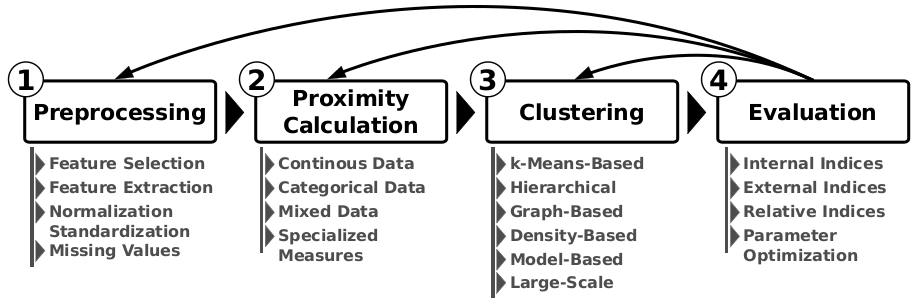
\includegraphics[scale=0.4]{./pictures/clusterAnalysis.png}
	\caption{Clustering overview of a cluster analysis \cite{clusterAnalysis}}
	\label{fig:clusterAnalysis}
\end{figure}

%%%%%%%%%%%%%%%%%%%%%%%%%%%%%%%%%%%%%%%%%%%%%%%%%%
\subsubsection{Preprocessing}
%%%%%%%%%%%%%%%%%%%%%%%%%%%%%%%%%%%%%%%%%%%%%%%%%%
A cluster analysis starts with the preparation of the data, which, in general, can be present in two forms \cite{clusterAnalysis}:
\begin{itemize}
	\item One-mode: A matrix of size $n \cdot n$. One-mode derives from the fact that rows and columns represents the same thing, the objects. The matrix describes the between-object relationship, and may be a distance or similarity matrix.
	\item Two-mode: Describes a $n \cdot p$ matrix, where \textit{n} is the objects and \textit{p} the features that describes the objects. This is also referred to as raw-data. One of the main challenges is converting the two-mode into one-mode by means of a suitable proximity function. All clustering tools require a method of relating the objects to each other. Tools working directly with two-mode data has an internal mechanism to obtain the between-object relationship.
	 \begin{figure}[H]
	 	\centering
	 	\[
	 	\texttt{X}
	 	=
	 	\begin{bmatrix}
	 	x_{11} & x_{12} & \dots & x_{1p} \\
	 	x_{21} & x_{22} & \dots & \dots \\
	 	\vdots & \vdots & \vdots & \vdots \\
	 	x_{n1} & \dots & \dots & x_{np}
	 	\end{bmatrix}
	 	\]
	 	\caption{Two-mode data matrix}
	 	\label{fig:dataMatrix}
	 \end{figure}
\end{itemize}

Presented with raw-data the features may be of different types which are \cite{clusteringOverview}:
\begin{itemize}
	\item Quantitative features which can be divided into:
		\begin{enumerate}
			\item Continuous values (e.g. fold changes of gene expressions)
			\item Discrete values (e.g. number of genes)
			\item Interval values (Timespan, 1-2 days)
		\end{enumerate}
	\item Qualitative features which can be divided into:
		\begin{enumerate}
			\item Nominal or unordered (e.g., eye-color)
			\item Ordinal (e.g., qualitative evaluations of pain: "no pain", "some pain")
		\end{enumerate}
	\item Structural data; Repeated measurements of the same variable under different conditions, e.g., time-series data of gene expression
\end{itemize}

Selecting the proper set of features is crucial. A given feature can have missing values or even outliers which can disturb the data. Imagine a feature which is uniformly at random distributed over the entire dataset. Such a feature is useless for identifying groups. The feature actually disturbs the process, and might blur the clusters into each other. In the other end a feature can be highly correlated and not yielding any additional information, which can bias the proximity calculations. The following methods can be distinguished of deriving a suitable set of features \cite{clusteringOverview}:
\begin{itemize}
	\item Feature Selection: Describes the task of selecting the most informative features for the clustering task. The goal of feature selection is the removal of irrelevant, redundant or noisy features, which serves the following objectives: (1) improve the cluster performance, (2) reduce the dataset size, (3) learn about the importance of the features, or (4) a combination of them \cite{22overview}. Usually feature selection is utilized for supervised learning. Considering the growing sizes of datasets it plays an important role for unsupervised learning as well. Reducing the number of features can potentially reduce the computation time. One challenge for feature selection is finding a balance between reducing the dataset while maintaining the structural information in the dataset.
	\item Feature Extraction: Describes methods which creates entirely new features based on the original features. The goals are similar to that of feature selection, reduction of the feature space to only the most relevant features. One frequently used method is the principal component analysis (PCA) \cite{26overview}. The idea is to transofrm the dataset to a reduced set of new uncorrelated features which retain most of the variation of the original dataset \cite{26overview}. Another common technique is the multidimensional scaling(MDS) which attempts an embedding of the objects into a lower-dimensional space while preserving the pairwise distances between objects as best as possible. Both methods are often used for data visualization by reducing the feature space to two or three dimensions.
\end{itemize}
There exists many additional feature manipulation techniques, also methods which expands the feature space, feature expansion \cite{33overview}.

Normalization or standardization is another vital step to preprocessing. The different scales might have a strong influence on the similarity function. When using the Euclidean distance, a feature may have distances ranging [0, 1], which will almost be disregarded when other features are in the millions \cite{33overview}. For which it might be crucial to normalize or standardize the features. The most common methods \cite{34overview, 35overview}:
\begin{itemize}
	\item Min-max normalization: Linear transformation of a feature to a predefined value range, normally between [0,1]
		\begin{equation}
			f' = \frac{f - \min_F}{\max_F - \min_F}
		\end{equation}
		$\min_F$ and $\max_F$ denotes the minimum and maximum of the feature F, and f represents some value of F.
	\item Autoscaling: Uses the standard deviation $\sigma_F$ of the values of F and the mean $\bar{F}$ to scale the variable
		\begin{equation}
			f' = \frac{f - \bar{F}}{\sigma_F}
		\end{equation}
	\item Decimal scaling: Describes the shifting of the radix point such that the largest value in the dataset is smaller than 1:
		\begin{equation}
			f' = \frac{f}{10^j}
		\end{equation}
		where \textit{j} is the smallest integer that that $\frac{\max_F}{10^j} < 1$.
\end{itemize}

A dataset may have missing values, which can derive from technical limitations, noise or error. Many similarity function cannot handle missing values, and removing incomplete objects or features may be an unacceptable solution. Treating missing values can be categorized as \cite{36overview}:
\begin{itemize}
	\item Prereplacing: Simply replace the missing values before usage. Methods to reconstruct can be the mean-and-mode method, nearest neighbor estimators or means of linear regression
	\item Embedded: Methods which attempts to handle missing values during the clustering process, thus allowing missing values in the dataset.
\end{itemize}

%%%%%%%%%%%%%%%%%%%%%%%%%%%%%%%%%%%%%%%%%%%%%%%%%%
\subsubsection{Proximity measures}
%%%%%%%%%%%%%%%%%%%%%%%%%%%%%%%%%%%%%%%%%%%%%%%%%%
Working with two-mode datasets, one important aspect of the cluster analysis is to establish a relationship between objects. The one-mode matrix is obtained via a proximity function, which either is a distance function or similarity function. Similarity function are maximal the more similar two objects are. The distance function are minimal the more similar two objects are. The choice of a suitable proximity function is highly dependent on the data types of the two-mode matrix. We will not go too much in depth with the following methods, but briefly mentioning for the sake of knowledge of existence.
\begin{itemize}
	\item Continuous Data: The common approaches for dealing with continuous data \cite{clusteringOverview}:
		\begin{itemize}
			\item Euclidean distance: The most common distance measure, which corresponds to the distance between two points measured with a ruler. Let $u = \{ u_1, \dots, u_p \}, v = \{v_1, \dots, v_p\} \in X$ be two objects with \textit{p} features:
				\begin{equation*}
					d(u, v) = \sqrt{\sum_{i = 1}^{p} (u_i - v_i) ^2}
				\end{equation*}
			\item Minkowski Distance: Which is the generalization of the Euclidean distance:
				\begin{equation*}
					d(u, v) = (\sum_{i = 1}^{p} | u_i - v_i|^l)^{\frac{1}{l}}
				\end{equation*}
				with the parameter \textit{l}. For $l = 2$ the Minkowski distance corresponds to the Euclidean distance. For $l = 1$ is corresponds to the Manhatten distance.
			\item Correlation: This method accounts for linear relationship between features. The Pearson correlation coefficient is defined as:
				\begin{equation*}
					\Phi(u, v) = \frac{\sum_{i = 1}^{p} (u_i - \bar{u})(v_i - \bar{v})}{\sqrt{\sum_{i = 1}^{p}(u_i - \bar{u}^2) \cdot \sum_{i = 1}^{p}(v_i - \bar{v})^2}}
				\end{equation*}
				The values range between [-1, 1]. The Pearson correlation is highest when the two features are perfectly linearly correlated
		\end{itemize}
		\item Categorical Data
			\begin{itemize}
				\item Boolean Variables: When comparing two objects \textit{u} and \textit{v} there are in total four possible outcomes, depicted in Figure \ref{fig:booleanVariables}. \textit{a} counts the number of positive matches. \textit{d} the number of negative matches. \textit{b} and \textit{c} the number of mismatches. Most measures define the similarity between objects by relating the number of matching features, \textit{a} and \textit{d}, to the number of mismatches, \textit{b} and \textit{c}.
					\begin{equation*}
						s(u, v) = \frac{a + d}{a + \lambda(b + c) + d}
					\end{equation*}
				For $\lambda = 1$ this corresponds to the Jaccard coefficient \cite{52overview}.
				\item General categorical variables: When dealing with categorical variables with more than two levels, different measures needs to be employed. One approach is deriving a score by counting the features for which the two objects agree:
				\begin{equation*}
				s(u, v) = \sum_{i = 1}^{p} \delta_k(u, v)
				\end{equation*}
				where $\delta_k(u, v)$ is the indicator function whether \textit{u} and \textit{v} are in the same category of feature \textit{k}.
			\end{itemize}
		\item Mixed Data Types: Describes a mixture of different data types, e.g., a mix of continuous and categorical features.
		\item Specialized Measures: Describes similarity functions which are specifically designed to a particular data type. In the fields of bioinformatics where a prominent one is NCBI BLAST \cite{blast}.
\end{itemize}
The choice of proximity function is crucial to the cluster analysis in terms of the clustering quality. Unfortunately there are no best-performer for all cases.

\begin{figure}
	\centering
	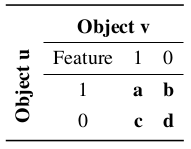
\includegraphics[scale=0.4]{./pictures/booleanVariables.png}
	\caption{Outcomes for boolean variables \cite{clusteringOverview}}
	\label{fig:booleanVariables}
\end{figure}

%%%%%%%%%%%%%%%%%%%%%%%%%%%%%%%%%%%%%%%%%%%%%%%%%%
\subsubsection{Clustering Strategies}
%%%%%%%%%%%%%%%%%%%%%%%%%%%%%%%%%%%%%%%%%%%%%%%%%%
The following strategies will only be mentioned briefly due to the scope of the project
\begin{itemize}
	\item k-means based: Algorithms which seek to identify an optimal \textit{k} clustering.
	\item Hierarchical: Clustering method which creates an entire nested tree structure of the clustering. In order to receive a specific clustering the tree is cut at a certain height to produce \textit{k} clusters. This method will be discussed in Section \ref{sec:hierarhicalClustering}.
	\item Graph-based: Algorithm the represents the data internally as a graph. The objects corresponds to the nodes, and the edges to the similarities between objects. Transitivity Clustering is a graph based strategy which we will discuss in Section \ref{sec:transClust}.
	\item Density-based: Approach which seeks to identify arbitrarily shapes clusters by separating high-density areas from low-density areas. Example of algorithms; DBSCAN and DENCLUE.
	\item Model-based: Clustering methods assume that the given dataset was generated by an underlying probabilistic method. THe aim is to maximize the model such that it best describes the observed data. Example of algorithms: Hidden-Markov-Model-based clustering, Self-Organizing Maps.
	\item Large-scale: Clustering methods in this category might belong to any of the above, but were developed to cope with large datasets. These are often running on distributed systems. Example of algorithms: BIRCH(Balanced Iterative Reducing and Clustering using Hierarchies), CURE(Clustering Using Representatives).
\end{itemize}

%%%%%%%%%%%%%%%%%%%%%%%%%%%%%%%%%%%%%%%%%%%%%%%%%%
\subsubsection{Clustering Properties}
%%%%%%%%%%%%%%%%%%%%%%%%%%%%%%%%%%%%%%%%%%%%%%%%%%
Whether a given tool is suitable or not cannot necessarily be derived solely based on the strategy of the clustering tool. The following properties should be considered given the compatibility of the clustering tool and the dataset \cite{64overview, 15overview}:
\begin{itemize}
	\item Scalability: Describes the behavior with increasing data set size in terms of runtime and memory consumptions.
	\item Dimensionality: The ability to handle the number of present features. Density-based clustering might be unable to discover any significant change of densities in data sets with very high dimensions, like gene expression data.
	\item Robustness: Describes the ability to cope with noise in the data. An algorithm which which reacts to small variations in the data with high variations in output may not be suitable. K-means is a tool which tend to react erratically in the presence of noise \cite{94overview}.
	\item Number of parameter and sensitivity: Describes the method's reliance on the user-input in tuning the algorithm. (1) The number of parameters should be as small as possible in order to avoid over-training of the algorithm. (2) It should be possible to anticipate the effect of the changing parameters, and not show near random effects on the clustering. E.g. small changes should not lead to big changes in the result. (3) The parameters should be interpretable. When the number of parameters increases it makes it difficult for a non-expert user.
	\item Arbitrary cluster shapes: The ability of the algorithm to identify arbitrarily shaped clusters.
	\item Usability and availability of the clustering tool is important. Most analyses are not carried out by computer experts, making a pure command-line tool error prone and could lead to maloperation.
\end{itemize}

%%%%%%%%%%%%%%%%%%%%%%%%%%%%%%%%%%%%%%%%%%%%%%%%%%
\subsubsection{Clustering Evaluation}
%%%%%%%%%%%%%%%%%%%%%%%%%%%%%%%%%%%%%%%%%%%%%%%%%%
One of the most critical steps in a cluster analysis is the evaluation of the clustering result. Clustering is a unsupervised learning without training data to guide, so how do we measure the quality? Evaluating two results can be difficult, if not impossible, when looking at plots of the clusterings. Thus, we need other methods to validate the results. \texttt{Cluster validity indices} are an important factor to evaluate solutions. There are three categories of validity indices \cite{onClustTechniques}
\begin{itemize}
	\item External validity indices : Evaluate the result with respect to a pre-specified structure, such as a gold standard. 
	\item Internal validity indices : Evaluate the result with respect to information intrinsic to the data alone.
	\item Relative validity indices: Choosing the best clustering scheme of a set of defined schemes, according to a pre-specified criterion.
\end{itemize}
Internal measures are often based on
\begin{itemize}
	\item Compactness: Measures how closely related the objects are in a cluster
	\item Separation: Measures how distinct or well-separated a cluster is from other clusters
\end{itemize}
Internal measures are e.g. Sum of Squares(SSQ), Silhouette Coefficient and Dunn Index. External measures use external information not present in the data. Normally a 'gold standard' is used. A gold standard is a clustering solution developed by experts, and are rarely available. In practice they are not available at all. Comparing against this ground truth is the way for determining the quality. External measures are e.g. F-measure and Jaccard coefficient. Generally, external validity indices evaluate a result in terms of the purity of individual clusters and the completeness of the clusters \cite{powerLimits}. Relative will not be further discussed, but an overview can be found in \cite{onClustTechniques}. There are many methods underlying these categories, but for the sake of brevity and the scope of the work, we limit ourselves to the F-measure. F-measure falls under the category of an external measure and will be discussed in Section \ref{sec:clusterValidation}.

%%%%%%%%%%%%%%%%%%%%%%%%%%%%%%%%%%%%%%%%%%%%%%%%%%
%%%%%%%%%%%%%%%%%%%%%%%%%%%%%%%%%%%%%%%%%%%%%%%%%%
%%%%%%%%%%%%%%%%%%%%%%%%%%%%%%%%%%%%%%%%%%%%%%%%%%
\newpage
\section{Background}
%%%%%%%%%%%%%%%%%%%%%%%%%%%%%%%%%%%%%%%%%%%%%%%%%%
%%%%%%%%%%%%%%%%%%%%%%%%%%%%%%%%%%%%%%%%%%%%%%%%%%
%%%%%%%%%%%%%%%%%%%%%%%%%%%%%%%%%%%%%%%%%%%%%%%%%%

%%%%%%%%%%%%%%%%%%%%%%%%%%%%%%%%%%%%%%%%%%%%%%%%%%
%%%%%%%%%%%%%%%%%%%%%%%%%%%%%%%%%%%%%%%%%%%%%%%%%%
\subsection{The Data}
%%%%%%%%%%%%%%%%%%%%%%%%%%%%%%%%%%%%%%%%%%%%%%%%%%
%%%%%%%%%%%%%%%%%%%%%%%%%%%%%%%%%%%%%%%%%%%%%%%%%%
We are using the Brown dataset \cite{brown}, which consists of 866 proteins(which we will refer to as the 'big dataset'). The dataset consists of 5 superfamilies: Amidohydrolase, Crotonase, Enolase, Haloacid dehalohenase and Vicinal uxygen chelate. A superfamily consists of a subset of families. The 5 superfamilies can be divided into a total of 91 families. We will be looking at the dataset in two sizes. The 'small dataset' consists of the Amidohydrolase superfamily which consists of 232 proteins, distributed over 29 families. We will be using both the big dataset and the small dataset throughout the project. Table \ref{brownTable} shows an overview of the superfamilies and the number of families in the entire Brown dataset. The information on number of families can be useful when looking at the clustering results. Clustering the small dataset, Amidohydrolase superfamily, the number of clusters in the optimal result should the same, or close to, the number of families, 29.

\begin{table}[]
	\centering
	\begin{tabular}{|l|c|}
		\hline
		Superfamily & Number of families \\\hline
		Amidohydrolase & 29 \\\hline
		Crotonase & 16 \\\hline
		Enolase & 9 \\\hline
		Haloacid dehalogenase & 20 \\\hline
		Vicinal oxygen chelate & 17 \\\hline
	\end{tabular}
	\caption{Overview of superfamilies and families in the Brown dataset}
	\label{brownTable}
\end{table}

%%%%%%%%%%%%%%%%%%%%%%%%%%%%%%%%%%%%%%%%%%%%%%%%%%
%%%%%%%%%%%%%%%%%%%%%%%%%%%%%%%%%%%%%%%%%%%%%%%%%%
\subsection{Transitivity Clustering}
\label{sec:transClust}
%%%%%%%%%%%%%%%%%%%%%%%%%%%%%%%%%%%%%%%%%%%%%%%%%%
%%%%%%%%%%%%%%%%%%%%%%%%%%%%%%%%%%%%%%%%%%%%%%%%%%
% article 'Comprehensive cluster analysis with Transitivity Clustering'
% article 'Partitioning biological data with transitivity clustering'
% article 'Large scale clustering of protein sequence with FORCE-A layout based heuristic for weighted cluster editing'
In this project we focus on Transitivity Clustering(TC). TC is a well proven algorithm which performs well on various tasks \cite{clustEval}, and is well suited for the plans we have.
Before going into any details about TC we need some basic graph-theoretic definitions \cite{extensionAndRobustnessTC}:
\begin{defn}[\texttt{Undirected simple graph}]\label{def:Undirected simple graph}
	An \texttt{undirected simple graph} $G = (V, E)$ consists of a set of nodes V and a set of edges $E \subseteq {V \choose 2}$, where ${V \choose 2}$ denotes the set of two-element subsets of V. The edges are undirected and contains no self-loops or multiple edges between two nodes. \textit{uv} is an unordered par $\{u, v \} \in {V \choose 2}$.
\end{defn}

\begin{defn}[\texttt{Transitive graph}]\label{def:Transitive graph}
	An undirected simple graph $G = (V, E)$ is called \texttt{transitive} 
	\begin{equation*}
	\text{if for all triples } uvw \in {V \choose 3}, uv \in E \text{ and } vw \in E \text{ implies } uw \in E.
	\end{equation*}
\end{defn}

\begin{defn}[\texttt{Weighted Transitive Graph Projection Problem(WTGPP)}]\label{def:WTGPP}
	 Given a set of objects \texttt{V}, a threshold $t \in \mathbb{R}$, and a pairwise similarity function sim: ${V \choose 2} \rightarrow \mathbb{R}$, the graph \textit{G} is defined as
	 \begin{equation}\label{eq:sim above threshold}
	 G = (V, E); \; E = \bigg\{ uv \in {V \choose 2} : \text{sim}(uv) > t\bigg\}
	 \end{equation}
	 The WTGPP is the determination of a transitive graph $G' = (V, E')$ such that there exist no other transitive graph $G'' = (V, E'')$ with $\text{cost}(G \rightarrow G'') < \text{cost}(G \rightarrow G')$. The modification costs are defined as
	 \begin{equation}\label{eq:TC cost function}
		 \text{cost}(G \rightarrow G') := \underbrace{\sum_{uv \in E \backslash E'} | \text{sim}(uv) - t |}_{\text{deletion cost}} + \underbrace{\sum_{uv \in E' \backslash E} | \text{sim}(uv) - t |}_{\text{addition cost}}
	 \end{equation}
\end{defn}

% Briefly write about the steps in the "algorithm" from article 'Comprehensive cluster analysis with trans clust'
% Talk about R package ????? (implementation section ?)

Transitivity Clustering takes one parameter, \textit{t}, which is the threshold for similarities. Following is the steps in Transitivity Clustering \cite{comprehensiveCAwithTC}:
\begin{enumerate}
	\item Model the given pairwise similarity, from the similarity matrix, as a similarity graph, \textit{G}. The nodes corresponds to the objects, with weighted edges as the similarity values.
	
	\item Transform the similarity graph, \textit{G}, into another graph, \textit{G'}, by subtracting the threshold from the edge weights. Subsequently removing those edges with weights below zero, which is the deletion cost for equation \ref{eq:TC cost function}.
	
	\item Transform \textit{G'} into a transitive graph, \textit{G''}, with minimal cost. Thus, in this step we add all edges such that the graph is transitive, which is the addition cost for equation \ref{eq:TC cost function}.
\end{enumerate}
The resulting transitive graph, \textit{G''}, is the clustering solution.


%%%%%%%%%%%%%%%%%%%%%%%%%%%%%%%%%%%%%%%%%%%%%%%%%%
%%%%%%%%%%%%%%%%%%%%%%%%%%%%%%%%%%%%%%%%%%%%%%%%%%
\subsection{Hierarchical Clustering}
\label{sec:hierarhicalClustering}
%%%%%%%%%%%%%%%%%%%%%%%%%%%%%%%%%%%%%%%%%%%%%%%%%%
%%%%%%%%%%%%%%%%%%%%%%%%%%%%%%%%%%%%%%%%%%%%%%%%%%
\begin{defn}[\texttt{Hierarchical Clustering(HC)} \cite{clusteringOverview}]\label{def:hc}
	Let N be the number of objects in the dataset. \\HC builds a nested structural partition of V, $H = \{ H_1, \dots, H_Q \} (Q \leq N$), such that $C_i \in H_m, C_j \in H_l$, and $m > l$ imply $C_i \in C_j$ or $C_i \cap C_j = \emptyset$ for all $i, j \neq i, l = 1, \dots, Q$.
\end{defn}

There are two forms of hierarchical Clustering, \texttt{agglomerative} and \texttt{divisive}. Agglomerate starts with \textit{n} clusters, where \textit{n} is the number of objects in the dataset. Joining clusters until one cluster is remaining, where all \textit{n} objects are members. Divisive is the opposite. Starting with one cluster with \textit{n} objects. Splitting the clusters until all clusters are singletons. Thus, all \textit{n} objects represents are cluster. Agglomerative is the most used, as divisive usually is a more expensive procedure. One important feature of hierarchical clustering is that a join or split of clusters are irrevocable, thus cannot be undone. Figure \ref{fig:agglo_vs_div} shows an overview of agglomerative vs. divisive.
\begin{figure}[H]
	\centering
	\includegraphics*[scale=0.3]{./pictures/hc/agglo_vs_div.png}
	\caption{Agglomerative vs. Divisive \cite{clusterAnalysis}.}
	\label{fig:agglo_vs_div}
\end{figure} 
The steps of joins or splits is often showed as a \texttt{dendrogram}, which is viewed as a tree structure. The root of the tree is the cluster containing all \textit{n} objects. Moving down the tree the nodes represents the clusters which was split from its parent. At the bottom of the tree we have the leafs, where the number of leafs represents all singleton clusters(the \textit{n} objects). The tree can be cut a given height resulting in a clustering solution. 

Figure \ref{fig:hc example} shows a \texttt{dendrogram} of the tree structure of a HC. The horizontal axis shows all the objects in the dataset. The vertical axis shows the distances between objects and/or clusters. Objects 1 and 2 are joined to a cluster at height 2. These are joined with the remaining objects at height 5, resulting in one cluster holding all objects.
\begin{figure}[H]
	\centering
	\includegraphics*[scale=0.3]{./pictures/hc/hc_example.png}
	\caption{Dendrogram of a Hierarchical Clustering \cite{clusterAnalysis}.}
	\label{fig:hc example}
\end{figure}

In a typical hierarchical Clustering the size and number of clusters are given by a threshold, much like the one used in \texttt{TC}. Meaning that one iteration can possibly affect all clusters, which either increases or decreases the overall quality. In Figure \ref{fig:hc example} the tree could be cut between distance 3-4 to obtain a solution containing three clusters.

%%%%%%%%%%%%%%%%%%%%%%%%%%%%%%%%%%%%%%%%%%%%%%%%%%
%%%%%%%%%%%%%%%%%%%%%%%%%%%%%%%%%%%%%%%%%%%%%%%%%%
\subsection{Cluster Validation}
\label{sec:clusterValidation}
%%%%%%%%%%%%%%%%%%%%%%%%%%%%%%%%%%%%%%%%%%%%%%%%%%
%%%%%%%%%%%%%%%%%%%%%%%%%%%%%%%%%%%%%%%%%%%%%%%%%%
We are using the brown dataset, which has a gold standard available. The F-measure uses a gold standard to measure the quality of a clustering, and thus falls under the category of an external measure. There are multiple versions of the F-measure. We will be using the F1-measure, where the measures Recall and Precision is weighted equally. F1-measure is the quasi-standard in clustering evaluation and has been proved useful in many biomedical contexts \cite{powerLimits}. From here on F1-measure will be stated as F-measure. Understanding the F-measure requires the following definitions \cite{powerLimits}:\\
$K = (K_1, \dots, K_m) = $ Clustering result obtained from the algorithm. $K_i$ is the \textit{i}'th cluster in \textit{K}.\\
$G = (G_1, \dots, G_l) = $ Gold standard clustering. $G_j$ is the \textit{j}'th cluster in \textit{G}.\\
$n = $ amount of objects in the dataset. \\
$n_i = $ number of objects in cluster $K_i$. \\
$n^j = $ number of objects in cluster $C_j$. \\
$n_{i}^{j} = $ number of objects contained in $K_i \cap C_j$

\begin{defn}[True Positive]\label{}
	The number of common objects between cluster \textit{i} and the compared gold standard cluster \textit{j}.
	\begin{equation}
		\text{TP} = |K_i \cap C_j|
	\end{equation}
\end{defn}

\begin{defn}[False Positive]\label{}
	The number of objects in cluster \textit{i}, which are not in the compared gold standard cluster \textit{j}.
	\begin{equation}
		\text{FP} = |K_i \backslash C_j|
	\end{equation}
\end{defn}

\begin{defn}[False Negative]\label{}
	The number of objects that are not in cluster \textit{i}, which are in the compared gold standard cluster \textit{j}
	\begin{equation}
		\text{FN} = |C_j \backslash K_i|
	\end{equation}
\end{defn}

\begin{defn}[Recall]\label{}
	\begin{equation}
		\text{Recall}(i,j) = \frac{n_{i}^{j}}{n_i} = \frac{TP}{TP + FP}
	\end{equation}
\end{defn}

\begin{defn}[Precision]\label{}
	\begin{equation}
		\text{Precision}(i,j) = \frac{n_{i}^{j}}{n^j} = \frac{TP}{TP + FN}
	\end{equation}
\end{defn}

\begin{defn}[F-measure for a cluster]\label{}
	The general F-measure for cluster \textit{j} and class \textit{i} is given by:
		\begin{equation}
			F_\beta (i, j) = \frac{(1 + \beta^2) \cdot \text{Precision}(i, j) \cdot \text{Recall}(i, j)}{(\beta^2 \cdot \text{Precision}(i, j)) + \text{Recall}(i, j)}
		\end{equation}
	As we are using the $F_1$-measure we can derive the following formula 
	\begin{equation}
		F(i,j) = 2 \cdot \frac{\text{Precision}(i,j) \cdot \text{Recall}(i,j)}{\text{Precision}(i,j) + \text{Recall}(i,j)}
	\end{equation}
\end{defn}

\begin{defn}[F-Measure for a clustering]\label{def:mean F-measure}
	In order to obtain the F-measure for a clustering solution, we need to find the mean F-measure. The F-measure of a cluster \textit{j} is multiplied by the amount of objects in the gold standard cluster which have most in common objects. Take the sum over all clusters. Divide by total amount of objects in the dataset. Each cluster from the gold standard can only be referenced/mapped once.
	\begin{equation}
		\frac{\sum_{i = 1}^{m} \text{F-measure}(K_i) \cdot n_{i}^{j}}{n}
	\end{equation}
\end{defn}
A F-measure is between 0 and 1. A value near 1 indicates a good match with the gold standard(good clustering result). Values near 0 indicates a bad result. It is important to pay attention to the statement in Definition \ref{def:mean F-measure} saying that each cluster from the gold standard can only be referenced once. If, e.g. three clusters from \textit{K} maps to the same clusters in \textit{C}, two clusters will be neglected. The F-measure will be 0.0 for the neglected clusters, which negatively influences the quality. This scenario can happen in all clustering solutions, but the probability for multiple mappings on to the same gold standard cluster increases when $|K|>|C|$. In the opposite direction the scenario where $|K|<|C|$, also has a negative impact. With $|K|<|C|$ the clusters in K would be bigger than the cluster in C. 
Looking back at Definition \ref{def:mean F-measure}, we see that the multiplication is done with the size of $C_j$. Therefore we can conclude that the amount of objects that $K_i$ is bigger than $C_j$, $|K_i|-|C_j|$, has a smaller influence on the total F-measure than the remaining objects in $K_i$.


%%%%%%%%%%%%%%%%%%%%%%%%%%%%%%%%%%%%%%%%%%%%%%%%%%
%%%%%%%%%%%%%%%%%%%%%%%%%%%%%%%%%%%%%%%%%%%%%%%%%%
\subsection{Multidimensional Scaling}
%%%%%%%%%%%%%%%%%%%%%%%%%%%%%%%%%%%%%%%%%%%%%%%%%%
%%%%%%%%%%%%%%%%%%%%%%%%%%%%%%%%%%%%%%%%%%%%%%%%%%
Preserving proper relationships between-object similarities is difficult when randomizing data. The randomization does not take into account that the similarities have to make any sense. E.g. think of having a dataset with two clusters, $c_1$ and $c_2$. Let $o_1$ be the point in the center of $c_1$. The randomization has made the similarities between $o_1$ and $c_1$ remain the same, but similarities between $o_1$ and $c_2$ has made $o_1$ the center point of $c_2$, following the similarities, while $c_1$ and $c_2$ have a low similarity. One solution is to change the similarities making $o_1$ a point between the two clusters, which alters the between-object similarities for the entire dataset. One way to preserve the between-object similarity as best as possible is to increase the number of dimensions, using multidimensional scaling \cite{powerLimits}. From the N-dimensional space of the dataset, the between-object distances can be calculated and a similarity matrix can be made. The resulting similarity matrix is the randomized version of the original data. One question that remains is what an appropriate number of dimensions would be, which will be covered in the Method section. The multidimensional scaling was done using a function in R, \textbf{isoMDS()} from the package \textbf{MASS}. The function requires as parameter a distance matrix, which is made from the similarity matrix with the Euclidean distance.


%%%%%%%%%%%%%%%%%%%%%%%%%%%%%%%%%%%%%%%%%%%%%%%%%%
%%%%%%%%%%%%%%%%%%%%%%%%%%%%%%%%%%%%%%%%%%%%%%%%%%
%%%%%%%%%%%%%%%%%%%%%%%%%%%%%%%%%%%%%%%%%%%%%%%%%%
\newpage
\section{Method}
%%%%%%%%%%%%%%%%%%%%%%%%%%%%%%%%%%%%%%%%%%%%%%%%%%
%%%%%%%%%%%%%%%%%%%%%%%%%%%%%%%%%%%%%%%%%%%%%%%%%%

%%%%%%%%%%%%%%%%%%%%%%%%%%%%%%%%%%%%%%%%%%%%%%%%%%
%%%%%%%%%%%%%%%%%%%%%%%%%%%%%%%%%%%%%%%%%%%%%%%%%%
\subsection{Assessing the best clustering}
\label{sec:bestClustering}
%%%%%%%%%%%%%%%%%%%%%%%%%%%%%%%%%%%%%%%%%%%%%%%%%%
%%%%%%%%%%%%%%%%%%%%%%%%%%%%%%%%%%%%%%%%%%%%%%%%%%
Assessing the quality of both datasets a test have been run for both where we increment the threshold by one for each run. Starting threshold($t_{\min}$) was set to -1, since the lowest similarity is 0. The -1 is to ensure that the first run has all proteins in one cluster. The maximum used threshold($t_{\max}$) is highest similarity + 1. The maximum similarity is not the same for the datasets. The small dataset has $t_{\max} = 324$, the big dataset has $t_{\max} = 181$. For the small dataset a similarity file was given. For the big dataset a BLAST output was given, where the similarities could be extracted by taking the $-log_{10}()$ of the values. BLAST(Basic Local Alignment Search Tool) is the most widely used method to search for sequence similarities \cite{blast}.

For the small dataset the optimal threshold was found to be 47 with a F-measure of 0.9816176. The same F-measure was given in the threshold range of 47-56. On \cite{clustEval} which has the quality measure for the same dataset, the optimal threshold was found to be 48.86 with F-measure 0.986. The measure from clusteval is approximately 0.004 higher than the implemented F-measure.
The testing has only been with thresholds as integers, and not decimals. Testing with threshold 48.86 did not give any better F-measure. The F-measure has been debugged several times, and there was not found any errors in the calculations. The optimal threshold for the big dataset was found to be 17 with F-measure 0.7647134. As earlier mentioned the different families in sequenced based homology protein dataset requires different thresholds for the optimum clustering, as the optimal threshold for the datasets reveals. \cite{partitioningBiologicalDataTC} Uses $F_2$-measure II, thus not exactly the same F-measure we are using. For the small dataset their findings was optimal threshold as 67 for the small dataset and 56 for the big dataset. 

%%%%%%%%%%%%%%%%%%%%%%%%%%%%%%%%%%%%%%%%%%%%%%%%%%
%%%%%%%%%%%%%%%%%%%%%%%%%%%%%%%%%%%%%%%%%%%%%%%%%%
\subsection{Transitivity-Hierarchical Clustering}
%%%%%%%%%%%%%%%%%%%%%%%%%%%%%%%%%%%%%%%%%%%%%%%%%%
%%%%%%%%%%%%%%%%%%%%%%%%%%%%%%%%%%%%%%%%%%%%%%%%%%
The Hierarchical Clustering with TC as the basis was implemented. The resulting dendrograms are similar to those returned by the hclust() method in R, thus making the implementation feasible. The first version of HC incrementally went through the range of threshold going from one cluster to all singleton clusters. An incrementation value for threshold can manually be set. An improved version was made where it is possible to enable binary search for a "good" threshold. Whenever the amount of splits at the given node are too many, it will try to find a more suitable, lower, threshold. Where the range of allowed splits, and incrementation of threshold is set manually. The binary search allows incrementation of bigger steps, while taking into account that the splits are not too many, which could lower the quality of the splits. The resulting dendrogram can be seen in Section \ref{result:hc}.  When testing with hclust() the agglomerative approach with \textit{complete linkage} was used. We implemented Hierarchical Clustering with the divisive approach and TC as the clustering algorithm. These differences has an impact on the dendrogram, as they work differently. Due to the scope of the project we will not explain how \textit{complete linkage} works.

%%%%%%%%%%%%%%%%%%%%%%%%%%%%%%%%%%%%%%%%%%%%%%%%%%
%%%%%%%%%%%%%%%%%%%%%%%%%%%%%%%%%%%%%%%%%%%%%%%%%%
\subsection{Randomization}
\label{sec:randomization}
%%%%%%%%%%%%%%%%%%%%%%%%%%%%%%%%%%%%%%%%%%%%%%%%%%
%%%%%%%%%%%%%%%%%%%%%%%%%%%%%%%%%%%%%%%%%%%%%%%%%%
For the randomization of the similarity matrix we need to preserve symmetry. Self-similarity is never queried, leaving the diagonal irrelevant. Let $D^i$ be the \textit{i}'th dimension in the D-dimensional space, where $D^i \in \{ x, y \}$ in the 2-dimensional space. Thus $D^i$ is the column vector for all values for the objects in dimension \texttt{i}. $D_{\min}^{i}$ is the minimum value, and $D_{\max}^{i}$ is the maximum value found in $D^i$.
We tested four different randomization approaches. In the results for each randomization approach we reason for the given approach and why it is feasible or infeasible. The reason for trying multiple randomization approaches is closely related to the results of the former approaches. The number indicates the version of the approach, where 1 is the first we tested, and 4 is the last.
The following are descriptions of all tested randomization approaches. Approach 2 through 4 are using multidimensional scaling.\\

\textbf{Approach 1}:
\begin{enumerate}
	\item Fill the upper matrix with randomly selected values from the actual similarity matrix. Diagonal is set to 0's.
	\item Make the matrix symmetric. The result is the random similarity matrix.
\end{enumerate}

\textbf{Approach 2}:
\begin{enumerate}
	\item Convert the actual similarity matrix into distances with the Euclidean distance.
	\item Scale from 2 dimensions into N dimensions with the isoMDS() method. Returned is the points in the N dimensional space.
	\item For all elements in $D^i$ randomly select a value in range $D_{\min}^{i} - D_{\max}^{i}$.
	\item Calculate the between-object distances.
	\item Conversion from distances to a similarity matrix, which is the resulting randomized similarity matrix.
\end{enumerate}

\textbf{Approach 3}:
\begin{enumerate}
	\item [1-5] Same steps as in approach 2.
	\item [6] Replace the lowest similarities in the matrix with 0's, matching the number of 0's in the actual similarity matrix.
\end{enumerate}

\textbf{Approach 4}:
\begin{enumerate}
	\item [1-5] Same steps as in approach 2.
	\item [6] Make an ordering of both matrices in ascending order.
	\item [7] Replace the i'th ordered element in actual similarity matrix with the i'th ordered element in the random similarity matrix, on the respective index in the random similarity matrix. Let [5,7] be the index of the i'th ordered similarity in random matrix. The value on index [5,7] will be replaced with the i'th ordered value from the actual similarity matrix.
	\item [8] Result is a randomized similarity matrix with the exact similarity distribution as the actual matrix.
\end{enumerate}

%%%%%%%%%%%%%%%%%%%%%%%%%%%%%%%%%%%%%%%%%%%%%%%%%%
%%%%%%%%%%%%%%%%%%%%%%%%%%%%%%%%%%%%%%%%%%%%%%%%%%
\subsection{Results}
%%%%%%%%%%%%%%%%%%%%%%%%%%%%%%%%%%%%%%%%%%%%%%%%%%
%%%%%%%%%%%%%%%%%%%%%%%%%%%%%%%%%%%%%%%%%%%%%%%%%%

%%%%%%%%%%%%%%%%%%%%%%%%%%%%%%%%%%%%%%%%%%%%%%%%%%
\subsubsection{Transitivity-Hierarchical Clustering}
%%%%%%%%%%%%%%%%%%%%%%%%%%%%%%%%%%%%%%%%%%%%%%%%%%
Figure \ref{fig:dendrogramHclustStandard} shows the dendrogram using the standard hierarchical clustering in R, hclust(). Figure \ref{fig:dendrogramHcImplemented} is the dendrogram from the implemented hierarchical clustering using TC as basis. A key note is that we are using the divisive approach where we move from one cluster to all singleton clusters. Therefore we are starting at the top of the dendrogram and moving downwards. Looking closer at both of the dendrograms we can see similar branches. For instance to the right in Figure \ref{fig:dendrogramHclustStandard} we see a large partition, this is one of the protein families with 100 proteins. In the left side of Figure \ref{fig:dendrogramHcImplemented} we notice a partition of the same size. The two partitions are in opposite sides, meaning that the ordering of the proteins on the x-axis are not the same. This does not influence the overall dendrogram as long as there are no overlapping branches. If there are any overlapping branches the ordering is suboptimal, since it makes the dendrogram more confusing. Looking more closely on both of the dendrograms we can find similar partitions, even though the splits are not on the same height. The big dataset has almost 4 times the proteins as the small dataset, making the branches of the dendrogram very dense. The dense branches makes it more difficult to analyze. The dendrograms for the big dataset are Figures \ref{fig:dendrogramHclustStandardBigData} and \ref{fig:dendrogramHcImplementedBigData}. The extension of TC into Hierarchical Clustering looks feasible from the resulting dendrograms. The difference in the dendrogram is most likely due to the underlying algorithms. The method hclust()(the standard implementation in R) uses the agglomerative approach with \textit{complete linkage} for the merging of objects and clusters. We are using the divisive approach with TC as the clustering method.

\begin{figure}[H]
	\centering
	\begin{minipage}{0.75\textwidth}
		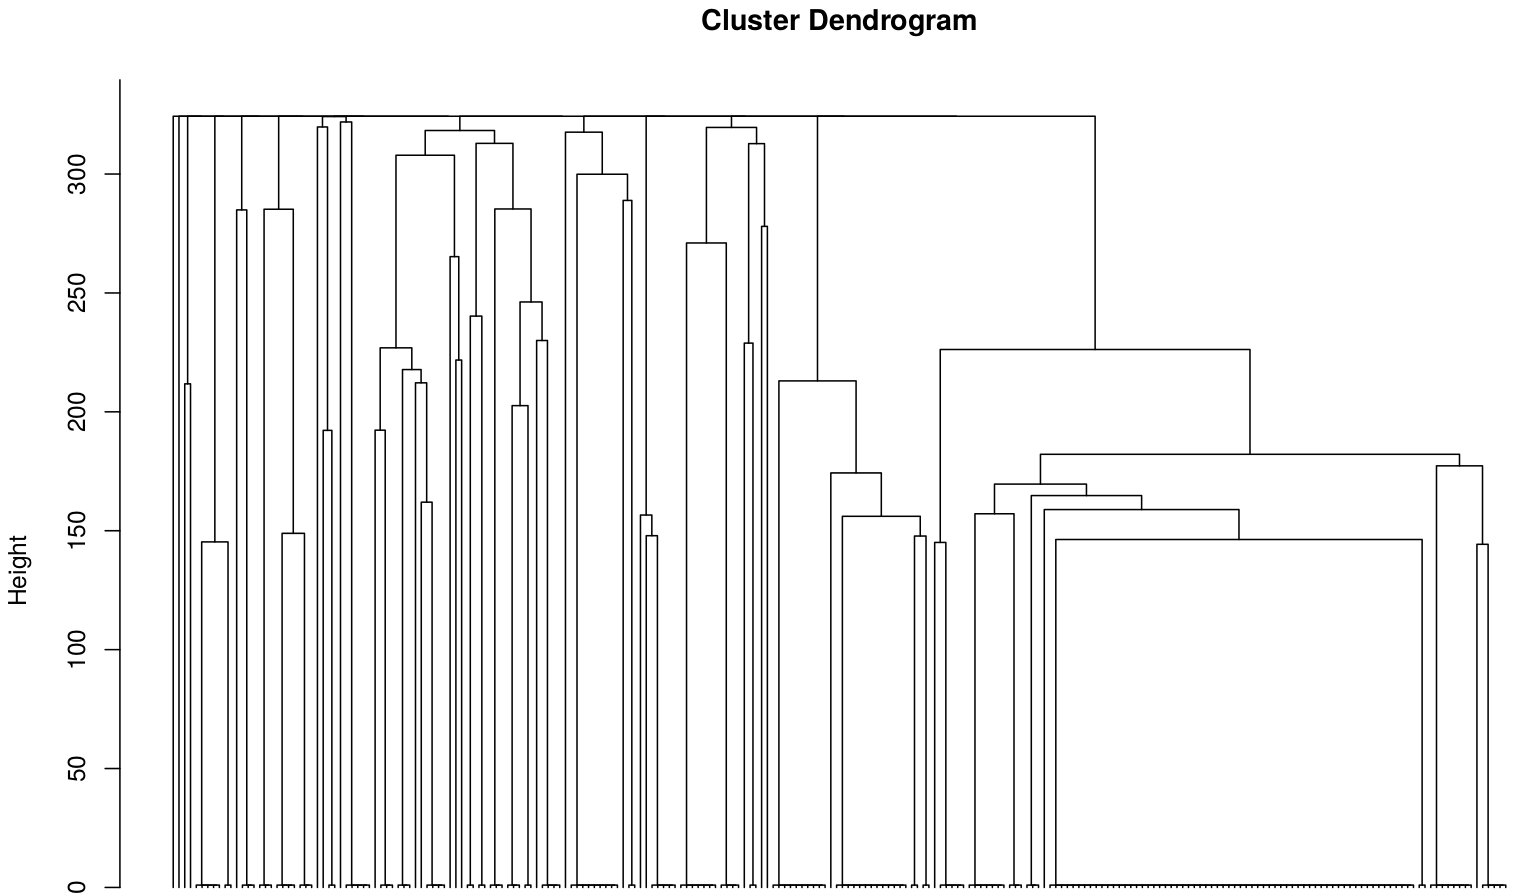
\includegraphics[width=1\textwidth]{./pictures/dendrogramHclustStandard.png}
		\caption{Resulting dendrogram with the small dataset - using the standard hclust() method in R}
		\label{fig:dendrogramHclustStandard}
	\end{minipage}
	\begin{minipage}{0.75\textwidth}
		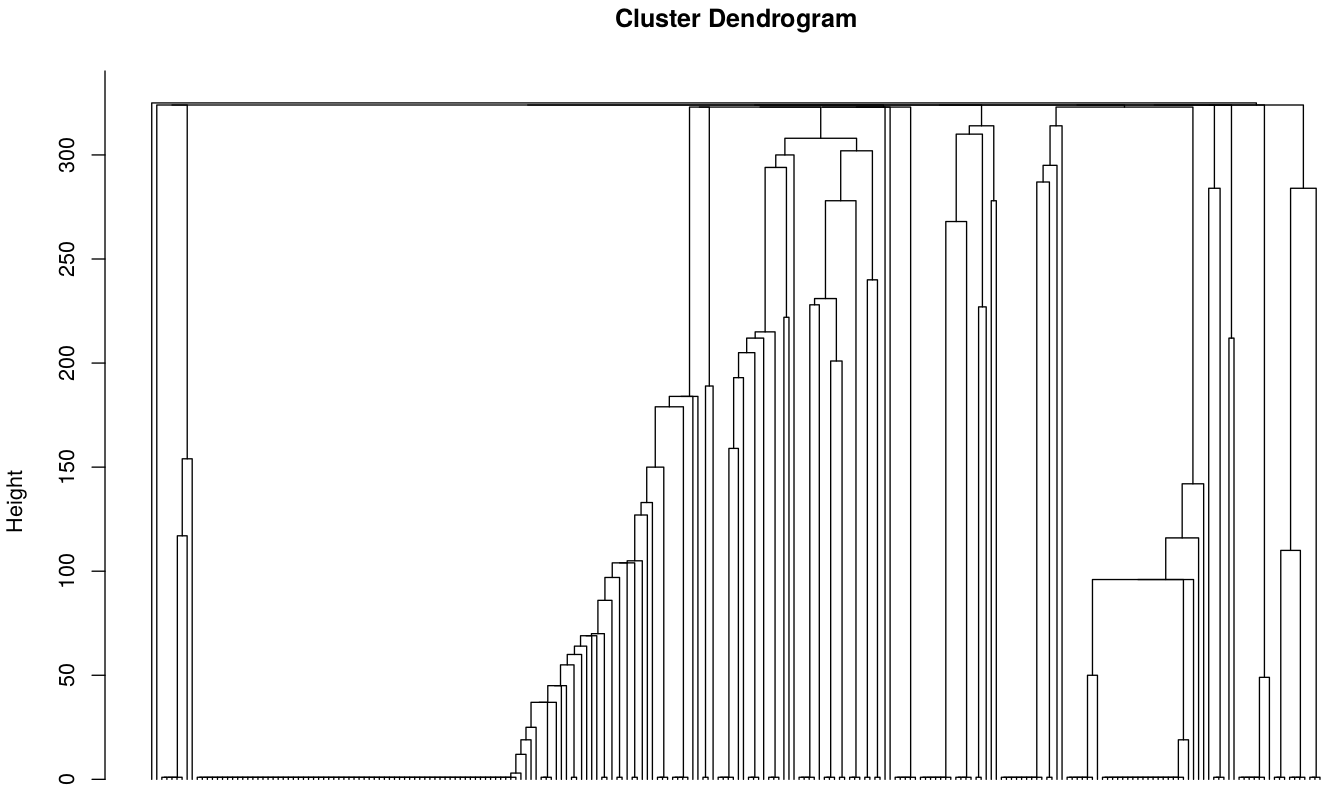
\includegraphics[width=1\textwidth]{./pictures/dendrogramHcImplemented.png}
		\caption{Resulting dendrogram with the small dataset - Implemented THC}
		\label{fig:dendrogramHcImplemented}
	\end{minipage}
\end{figure}

\begin{figure}[H]
	\centering
	\begin{minipage}{0.75\textwidth}
		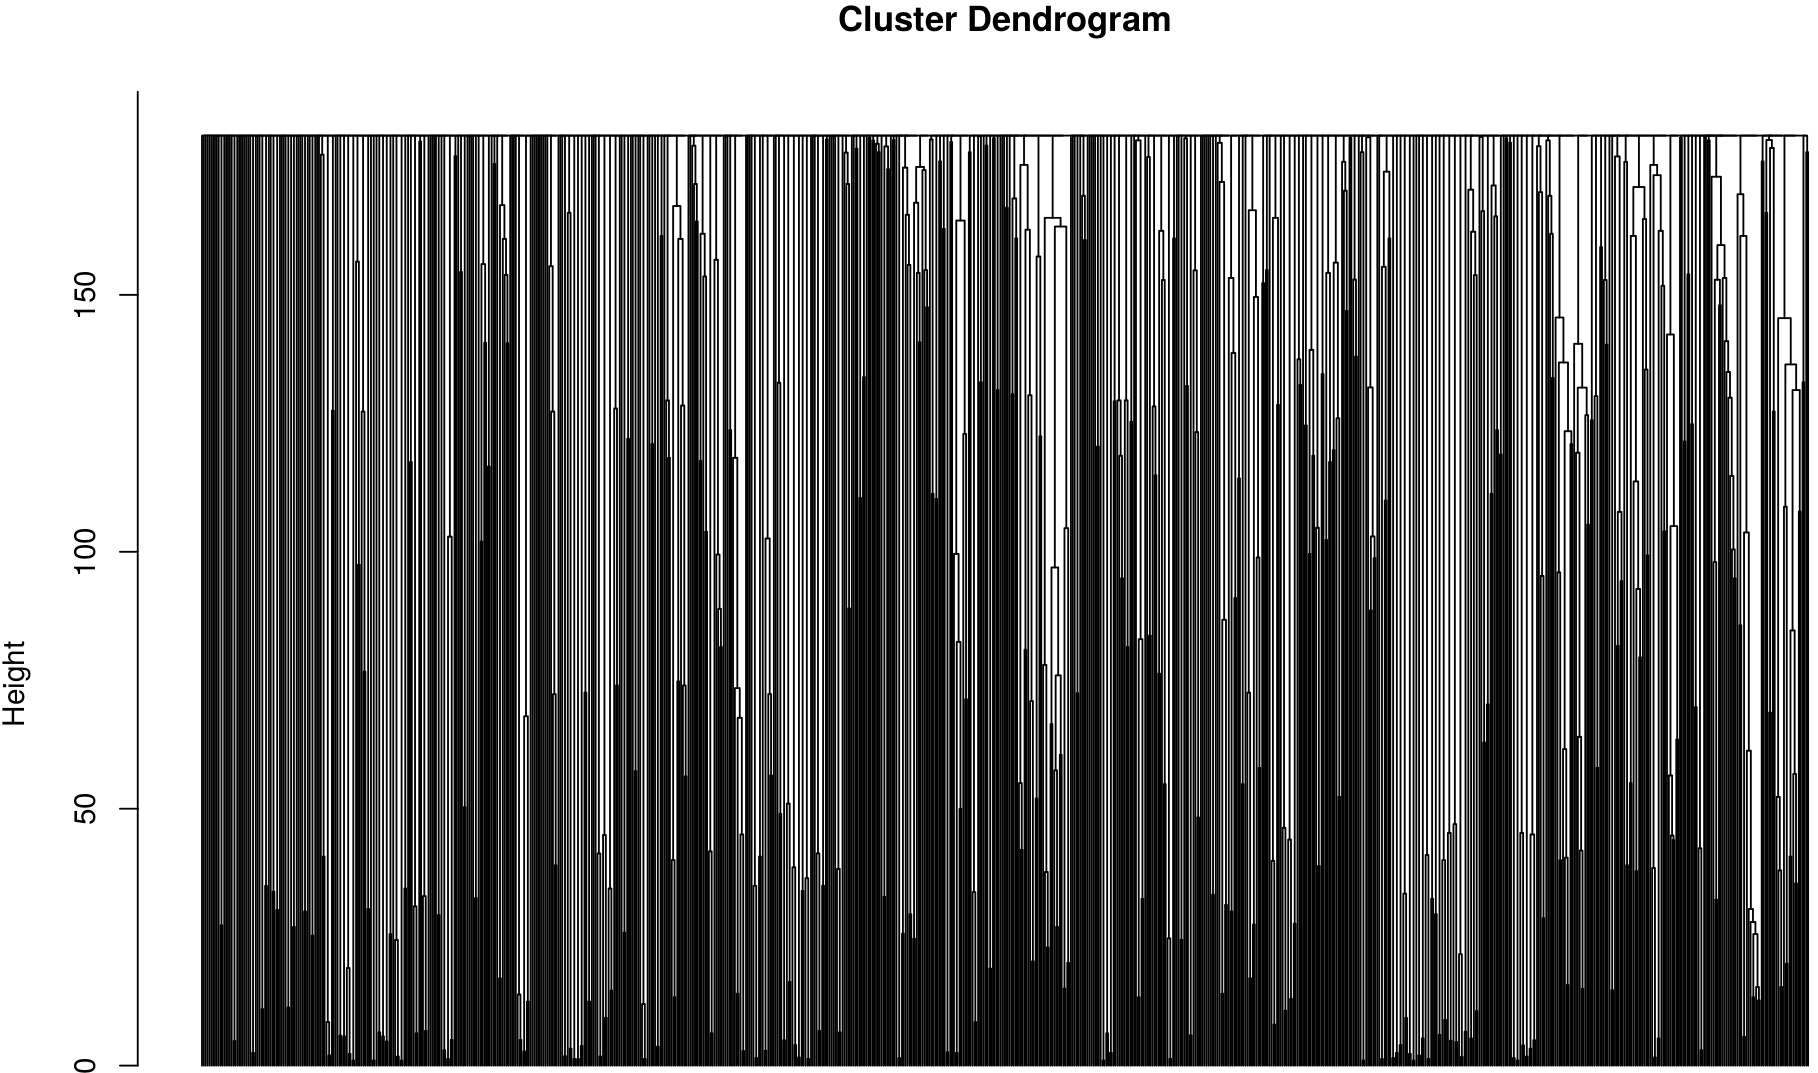
\includegraphics[width=1\textwidth]{./pictures/dendrogramHclustBigData.png}
		\caption{Resulting dendrogram with the big dataset - using the standard hclust() method in R}
		\label{fig:dendrogramHclustStandardBigData}
	\end{minipage}
	\begin{minipage}{0.75\textwidth}
		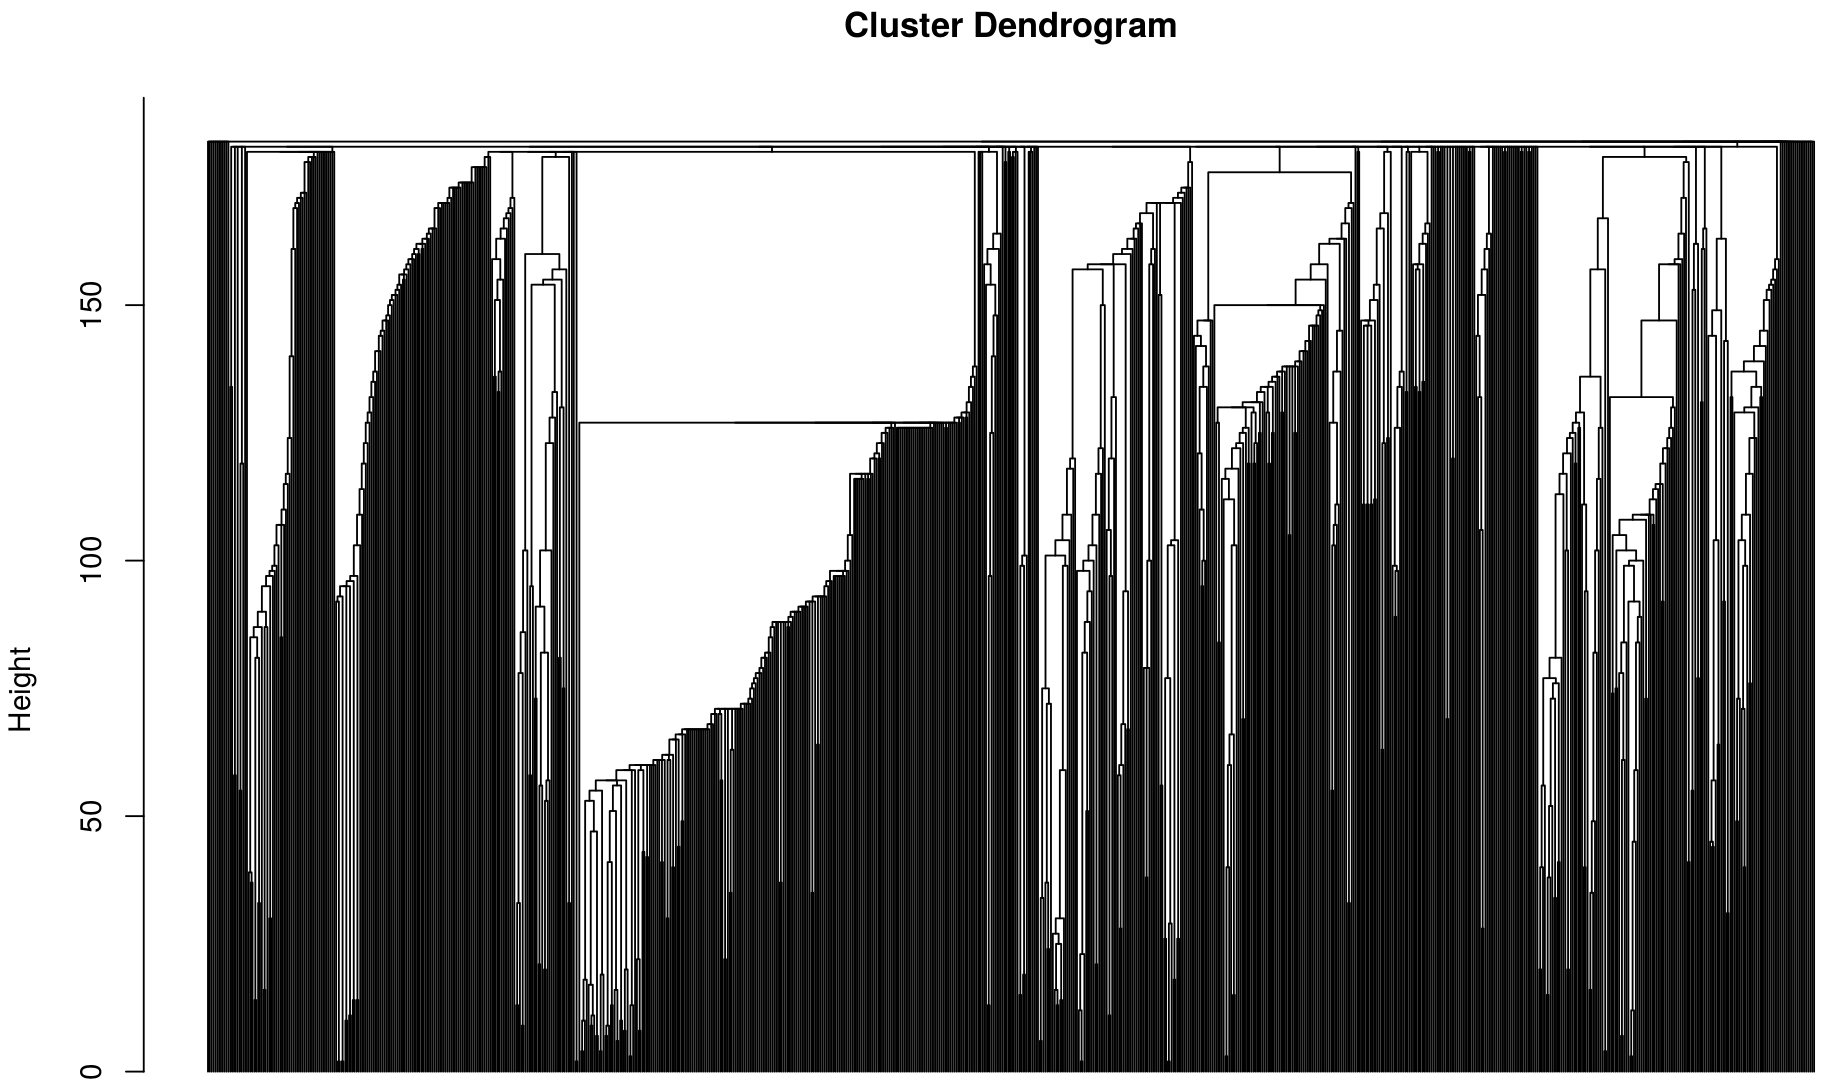
\includegraphics[width=1\textwidth]{./pictures/dendrogramBigDataHcImplemented.png}
		\caption{Resulting dendrogram with the big dataset - Implemented THC}
		\label{fig:dendrogramHcImplementedBigData}
	\end{minipage}
\end{figure}

%%%%%%%%%%%%%%%%%%%%%%%%%%%%%%%%%%%%%%%%%%%%%%%%%%
\subsubsection{Randomization}
%%%%%%%%%%%%%%%%%%%%%%%%%%%%%%%%%%%%%%%%%%%%%%%%%%
As mentioned in Section \ref{sec:randomization} we have tested four different randomization approaches where the results are in the following sections.
For the actual datasets the costs for the different threshold in the range of $t_{\min}$ to $t_{\max}$ is given by figures \ref{fig:measureSmallData} and \ref{fig:measureBigData}. As we can see the small dataset peaks at approximately 60,000. The big dataset peaks at approximately 680,000. 
Each dataset has a $t_{\min}$ and a $t_{\max}$. These were defined for the small and big dataset in Section\ref{sec:bestClustering}. For the randomized dataset they correspond to:
\begin{itemize}
	\item $t_{\min}$: The lowest similarity in the dataset where we subtract 1. For all datasets it has been found $t_{\min} = -1$.
	\item $t_{\max}$: The highest similarity in the dataset where we add 1. No guarantee for this to be the same as for the small or big dataset, depending on which was randomized. Although $t_{\max}$ for the random big dataset seems to be the same as for the actual data, which the cost plots will show in the the following sections.
\end{itemize}
\begin{figure}
	\centering
	\begin{minipage}{0.75\textwidth}
		\centering
		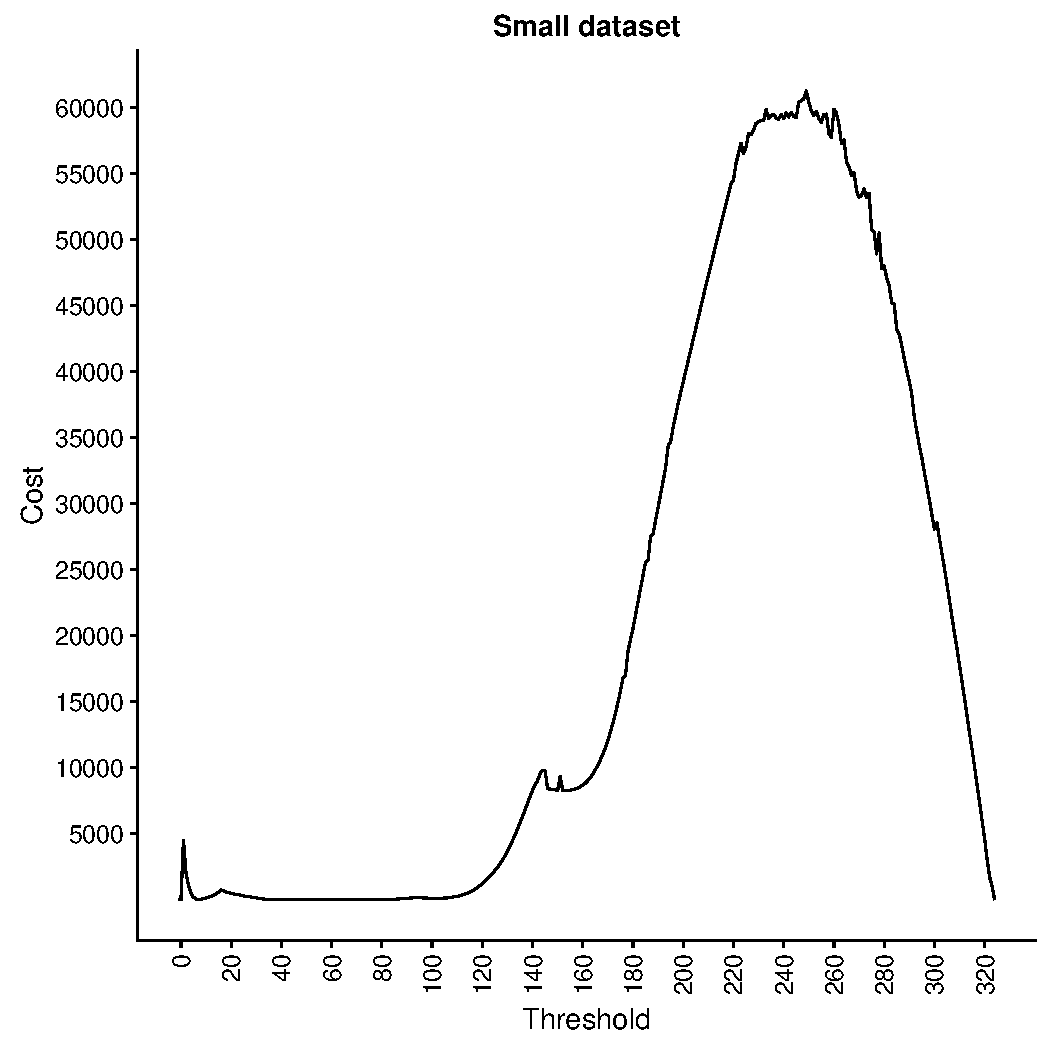
\includegraphics[width=0.9\textwidth]{./plots/plotCostSmallDataOriginal.pdf}
		\caption{Clustering costs returned by TC}
		\label{fig:measureSmallData}
	\end{minipage}
	\begin{minipage}{0.75\textwidth}
		\centering
		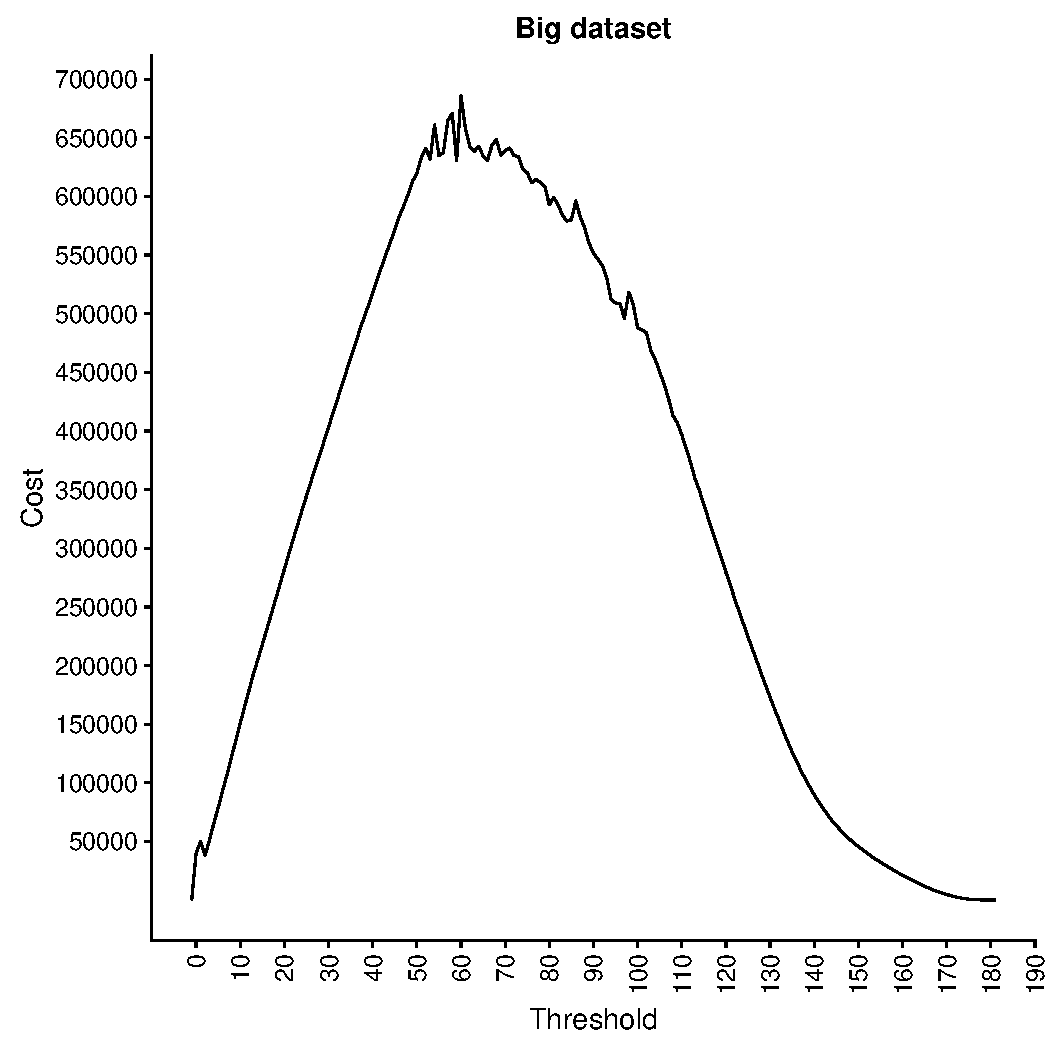
\includegraphics[width=0.9\textwidth]{./plots/plotCostBigDataOriginal.pdf}
		\caption{Clustering costs returned by TC}
		\label{fig:measureBigData}
	\end{minipage}
\end{figure}


%%%%%%%%%%%%%%%%%%%%%%%%%%%%%%%%%%%%%%%%%%%%%%%%%%
\subsubsection{Randomization Approach 1}
%%%%%%%%%%%%%%%%%%%%%%%%%%%%%%%%%%%%%%%%%%%%%%%%%%
Requiring the cost for the randomized dataset the range $t_{\min}$ to $t_{\max}$ was tested with incrementation of 1. This approach turned out as misleading, as the costs for the random data peaked at 1,000,000, which is far from the actual data of 60,000. Multiple randomizations was tested, leaving the same high costs above 1,000,000. Reasons for the high costs are due to the between-object similarities, as discussed in the section Multidimensional Scaling. There is no structure in the random data, which is the cause of the high costs. As the results was misleading for the small dataset the big dataset was not tested.


%%%%%%%%%%%%%%%%%%%%%%%%%%%%%%%%%%%%%%%%%%%%%%%%%%
\subsubsection{Randomization Approach 2}
%%%%%%%%%%%%%%%%%%%%%%%%%%%%%%%%%%%%%%%%%%%%%%%%%%
The costs for approach 1 was tremendously high compared to the actual data, which lead to a randomization utilizing multidimensional scaling. Multidimensional scaling was used to increase the number of dimensions. In this higher dimensional space, the points was randomized, where we derived similarities. This approach was tested with dimensions in the range of 5-100 with steps of 5. In order to obtain the costs for the randomized data TC was run with threshold in the range of $t_{\min}$ to $t_{\max}$. 
For the small dataset we randomized once for each dimension, giving a sample size of 20 runs. The costs are peaking in the range 190,000-320,000 across the range of dimensions, see Figure \ref{fig:plotCostsRandomSmallDataAp2}. As this is an improvement compared to approach 1, it was tested with the big dataset. For the big dataset we randomized four times for each dimension, resulting in a sample size of 80 runs. The costs for the small dataset has decreased significantly. Here the peaks of costs are in the range of 2,000,000-3,100,000, shown in Figure \ref{fig:plotCostsRandomBigDataAp2}. For both datasets the costs of the random dataset are in the range of 3-6 times higher than the actual data. For all the tested dimensions the biggest gap is where the cost for the random data is peaking, or very close to the peak. This is shown in figures \ref{fig:maxGapCostBigDataAp2K5} and \ref{fig:maxGapCostBigDataAp2K10}. The influencer of the biggest gap is simply where the cost is peaking in the randomized data. Therefore we cannot derive any useful information with this approach. Utilizing multidimensional scaling has not improved the randomization well enough in terms of the structure of the data.

\begin{figure}[H]
	\centering
	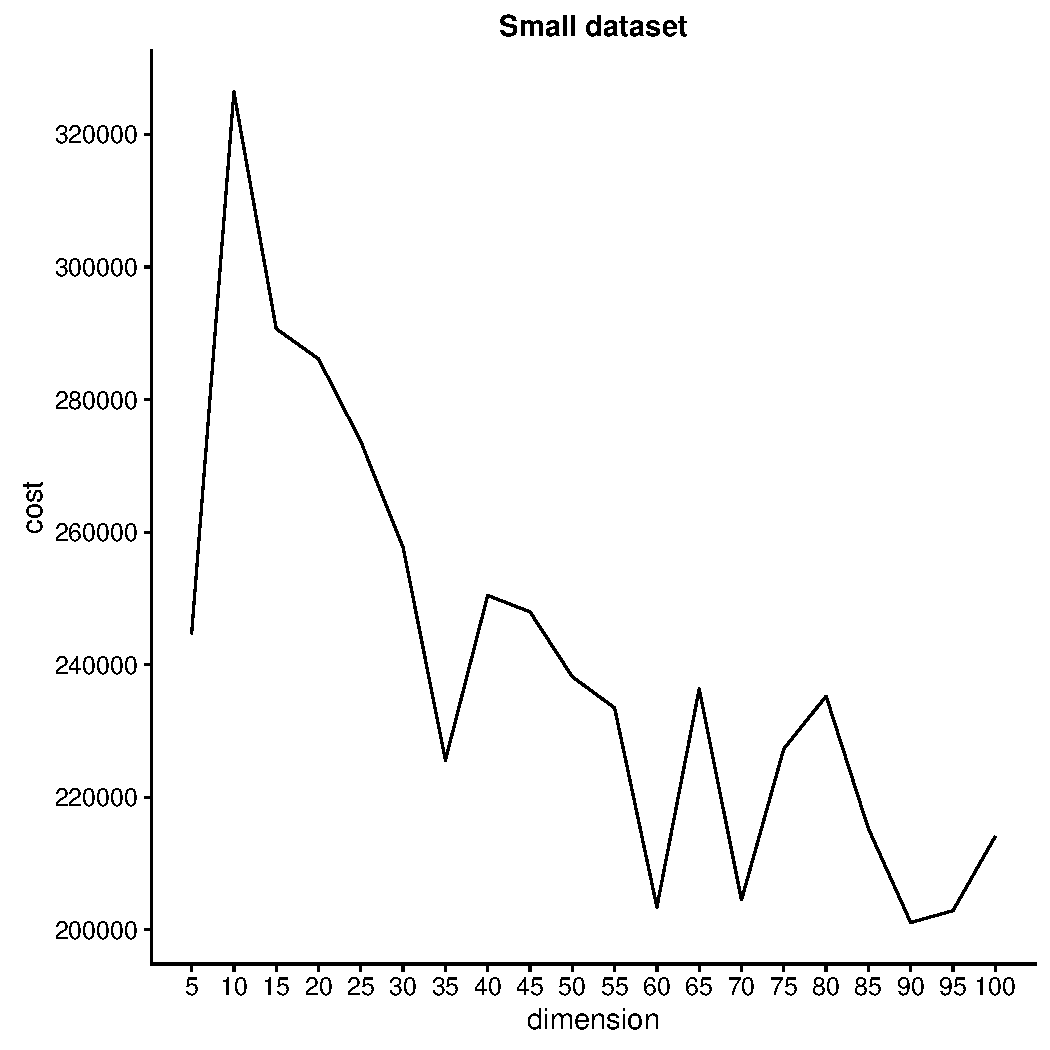
\includegraphics[width=0.8\textwidth]{./plots/plotCostsRandomSmallData-Ap2.pdf}
	\caption{Randomization approach 2: Max cost distribution across dimensions. The costs returned by TC with threshold in the range of $t_{\min}$ to $t_{\max}$. The threshold was incremented by 1 for each run.}
	\label{fig:plotCostsRandomSmallDataAp2}
\end{figure}

\begin{figure}[H]
	\centering
	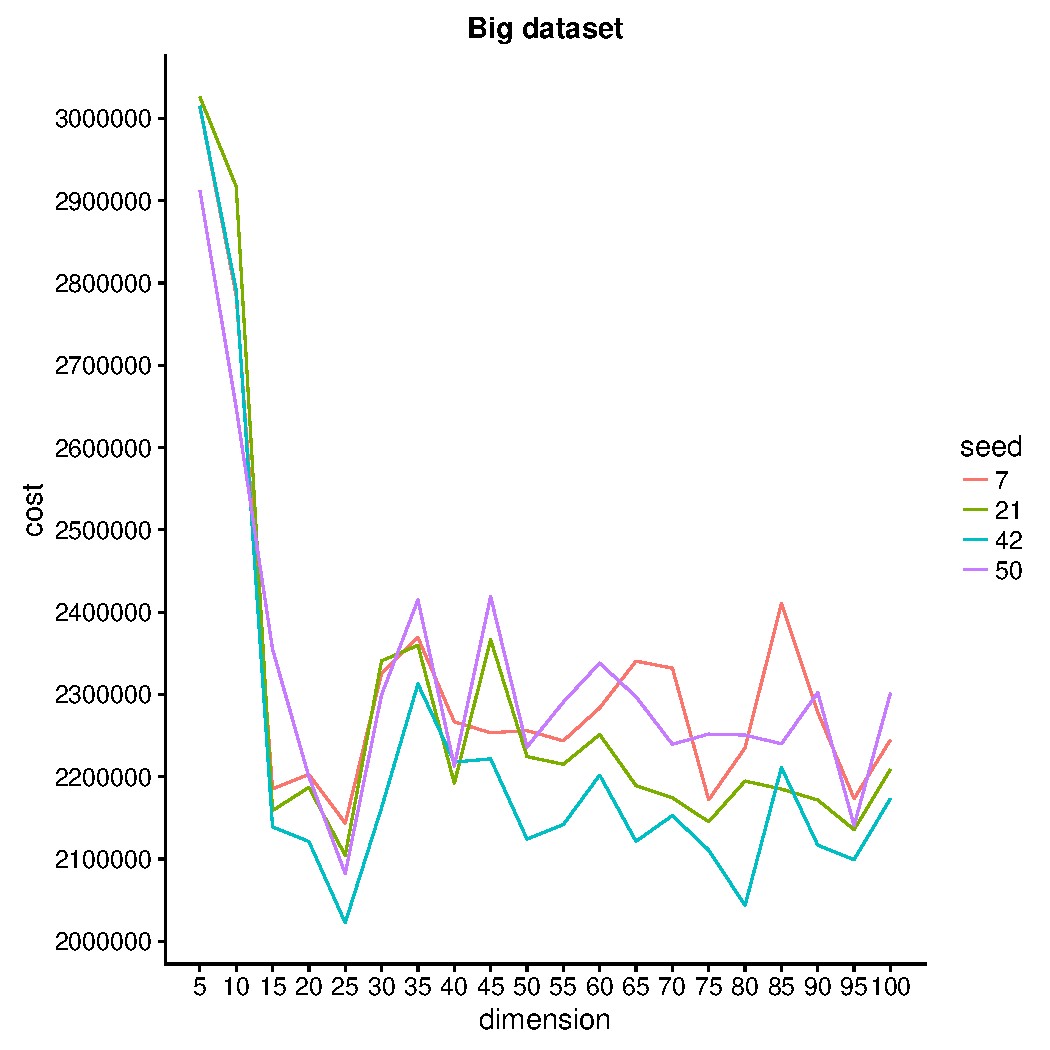
\includegraphics[width=0.8\textwidth]{./plots/plotMaxCostRandomBig/plotCostsRandomBigData-Ap2.pdf}
	\caption{Randomization approach 2: Max cost distribution across dimensions. The costs returned by TC with threshold in the range of $t_{\min}$ to $t_{\max}$. The threshold was incremented by 1 for each run.}
	\label{fig:plotCostsRandomBigDataAp2}
\end{figure}

\begin{figure}[H]
	\centering
	\begin{minipage}{0.75\textwidth}
		\centering
		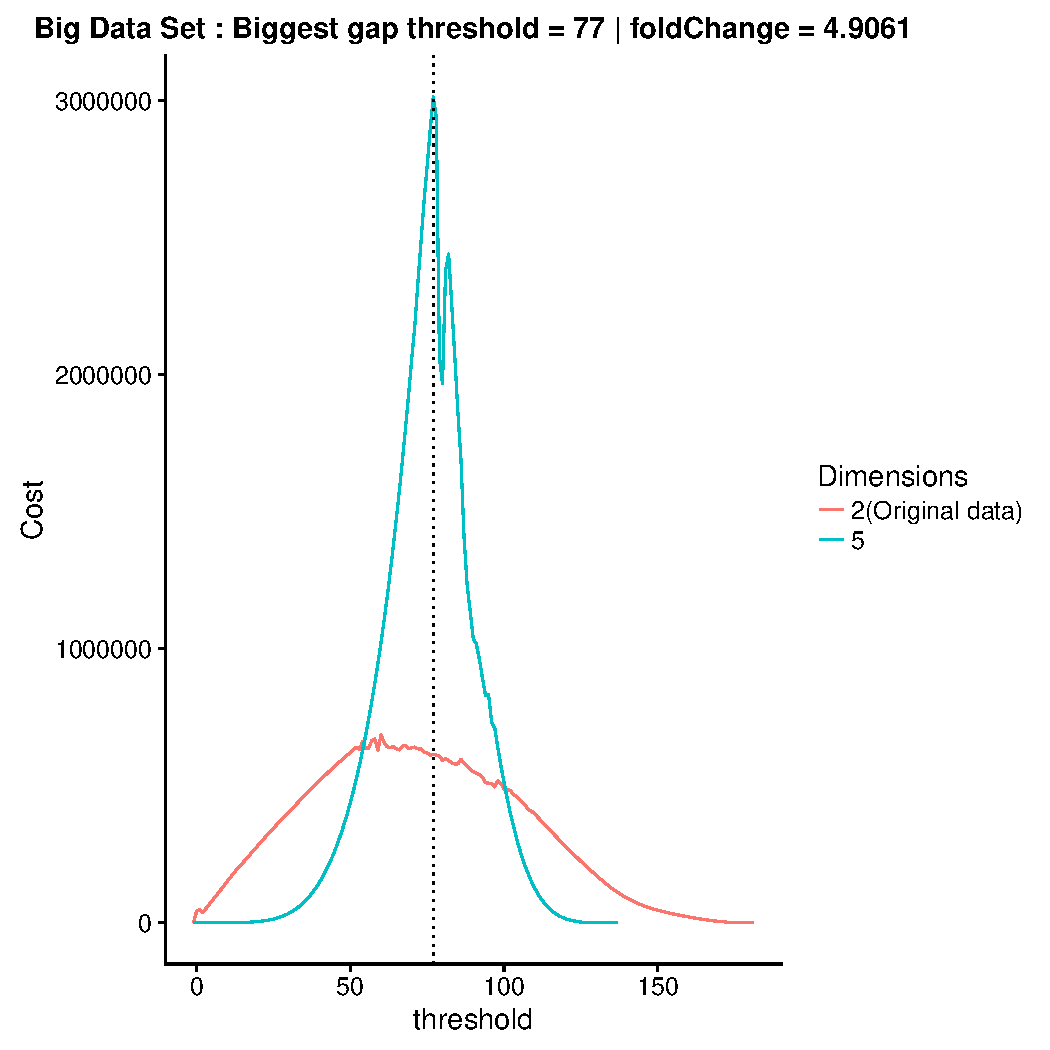
\includegraphics[width=0.9\textwidth]{./plots/plotsCostAndSimAp234/plotBigDataCostAndSim-AP2-S7-K5.pdf}
		\caption{Randomization approach 2: Max gap cost}
		\label{fig:maxGapCostBigDataAp2K5}
	\end{minipage}
	\begin{minipage}{0.75\textwidth}
		\centering
		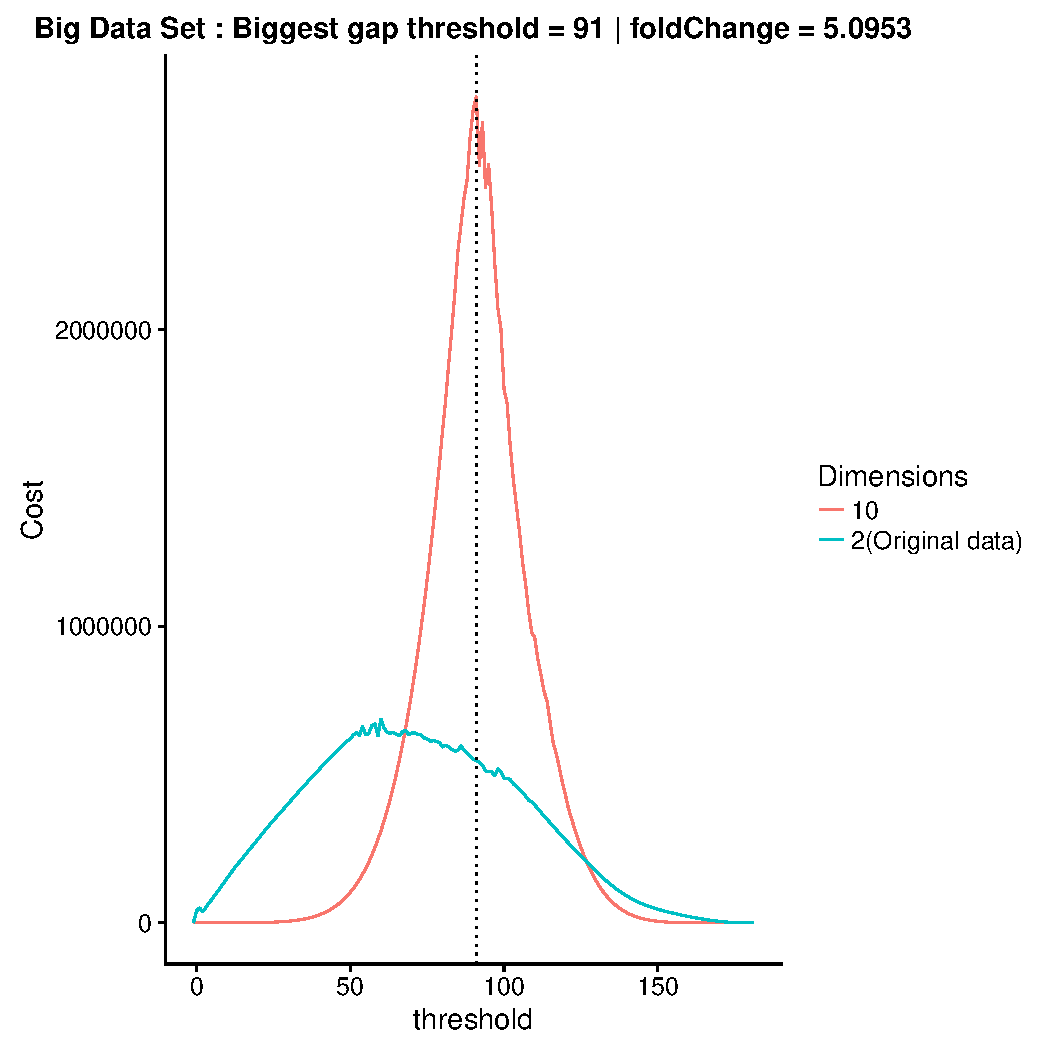
\includegraphics[width=0.9\textwidth]{./plots/plotsCostAndSimAp234/plotBigDataCostAndSim-AP2-S7-K10.pdf}
		\caption{Randomization approach 2: Max gap cost}
		\label{fig:maxGapCostBigDataAp2K10}
	\end{minipage}
\end{figure}

%%%%%%%%%%%%%%%%%%%%%%%%%%%%%%%%%%%%%%%%%%%%%%%%%%
\subsubsection{Randomization Approach 3}
%%%%%%%%%%%%%%%%%%%%%%%%%%%%%%%%%%%%%%%%%%%%%%%%%%
The costs for the randomized data was obtained the same way as we did with approach 4. From the results of testing many different dimensions with approach 2, we concluded it was enough to test the dimensions 2, 3, 4, 5 and 10 from here on. Each dimension was randomized four times, giving a sample size of 20 runs. Figure \ref{fig:plotCostsRandomBigDataAp3} shows the distribution of the highest cost across the tested dimensions. The distribution looks better than the one in approach 2, Figure \ref{fig:plotCostsRandomBigDataAp2}. The cost is starting in the lower end with the lower dimensions. From dimension 30 the cost stays within a range of 500,000. Looking at Figure \ref{fig:maxGapCostBigDataAp3K5} it shows similar results as approach 2, where the biggest gap is at the peak of the random data. In 16/20 the biggest gap is at the highest peak of the random data. The remaining 4 tests has the biggest gap outside of the peak of the random data. Figure \ref{fig:maxGapCostBigDataAp3K2} shows a promising result. The max gap is at threshold 17, which is the exact same threshold which gave the best clustering quality according to the F-measure. One thing to notice is that this result is from a random dataset with 2 dimensions. For the remaining 3 that has the biggest gap outside the peak, the gap is at thresholds 9(2 dimensions), 10(5 dimensions) and 14(2 dimensions). Although this approach looks looks promising, we wanted to try another approach. Hitting the biggest way from the peaking cost in 4/20 of the tests is not by any means an impressive statistic. If this statistic would hold, we need to randomize and run TC on a given dataset 5 times. Including the run for the actual data, thus a total of 6 clusterings.

\begin{figure}[H]
	\centering
	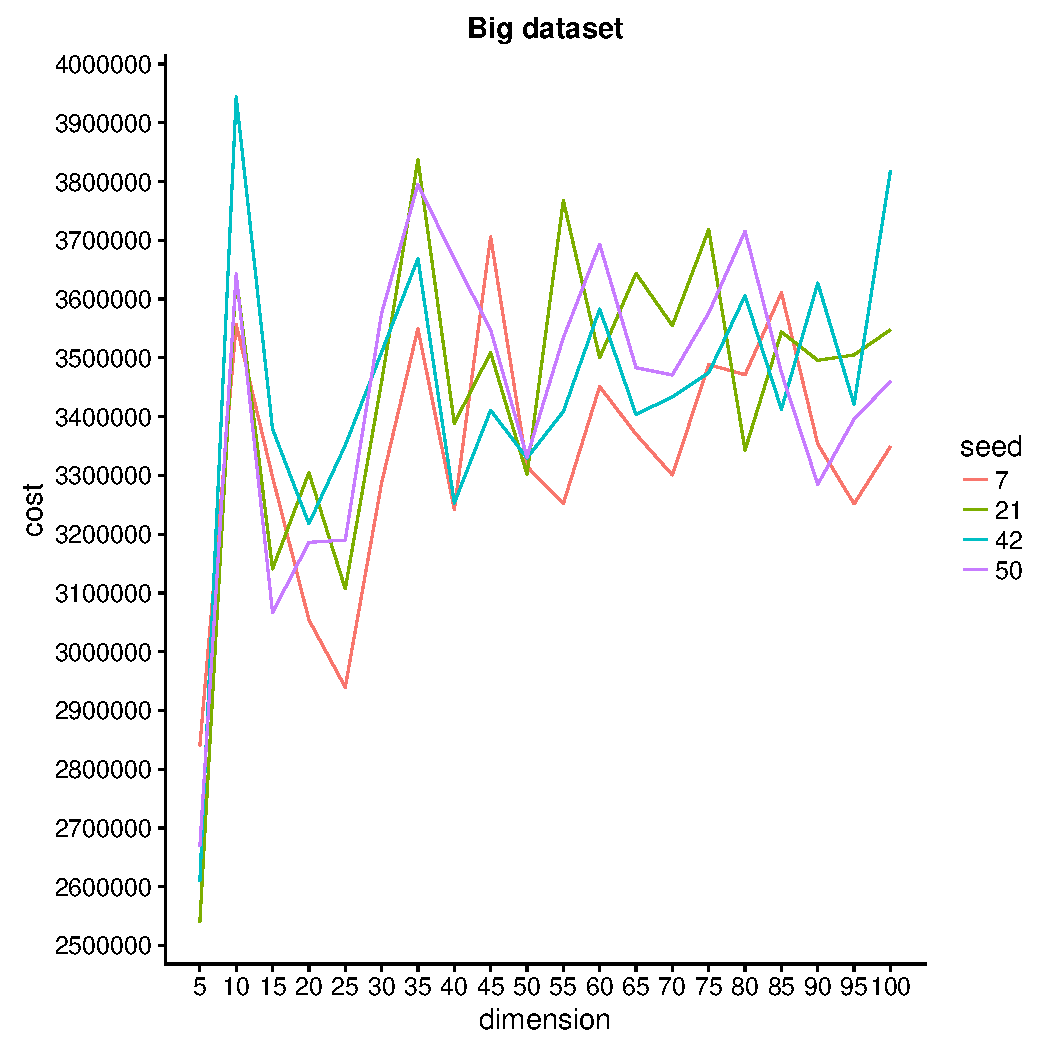
\includegraphics[width=0.8\textwidth]{./plots/plotMaxCostRandomBig/plotCostsRandomBigData-Ap3.pdf}
	\caption{Randomization approach 3: Max cost distribution across dimensions}
	\label{fig:plotCostsRandomBigDataAp3}
\end{figure}

\begin{figure}[H]
	\centering
	\begin{minipage}{0.75\textwidth}
		\centering
		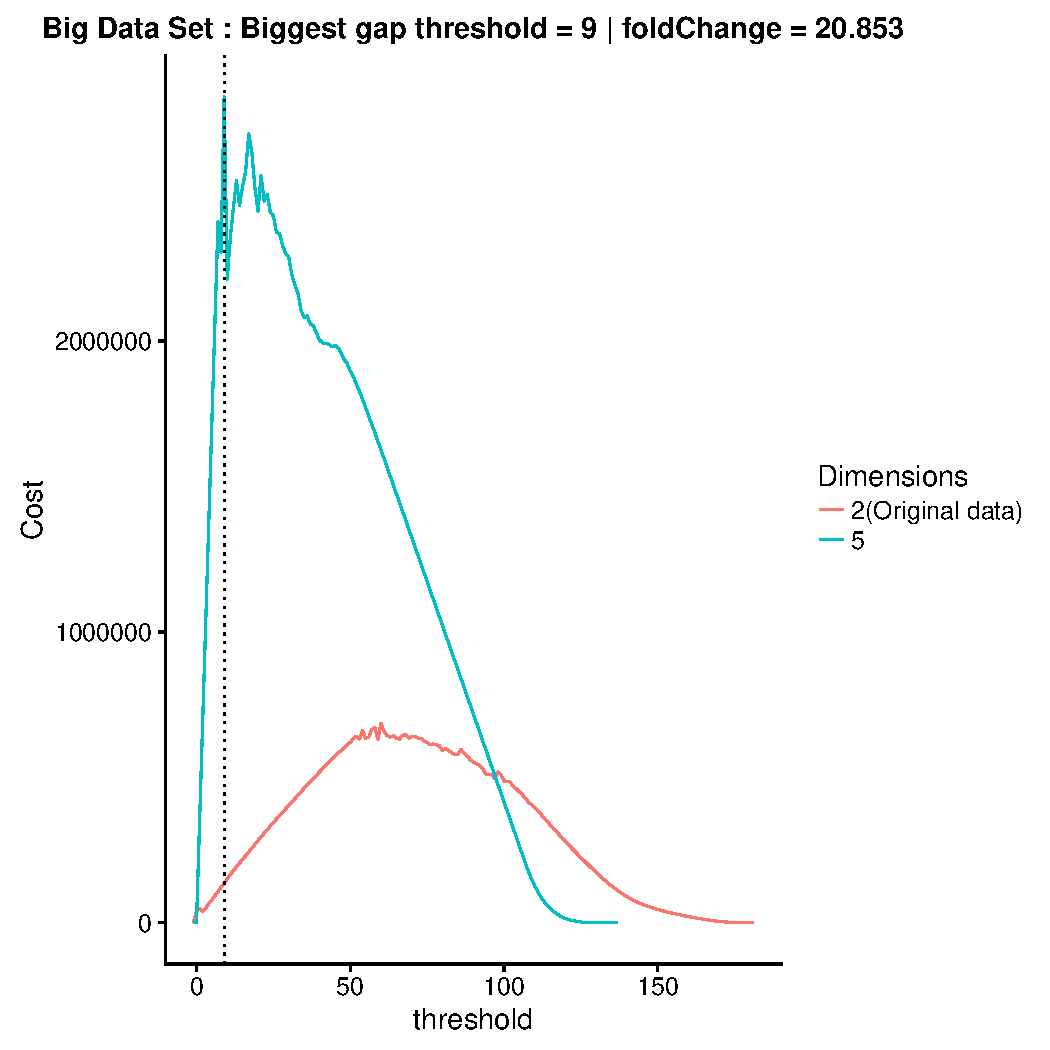
\includegraphics[width=0.9\textwidth]{./plots/plotsCostAndSimAp234/plotBigDataCostAndSim-AP3-S7-K5.pdf}
		\caption{Randomization approach 3: Max gap cost}
		\label{fig:maxGapCostBigDataAp3K5}
	\end{minipage}
	\begin{minipage}{0.75\textwidth}
		\centering
		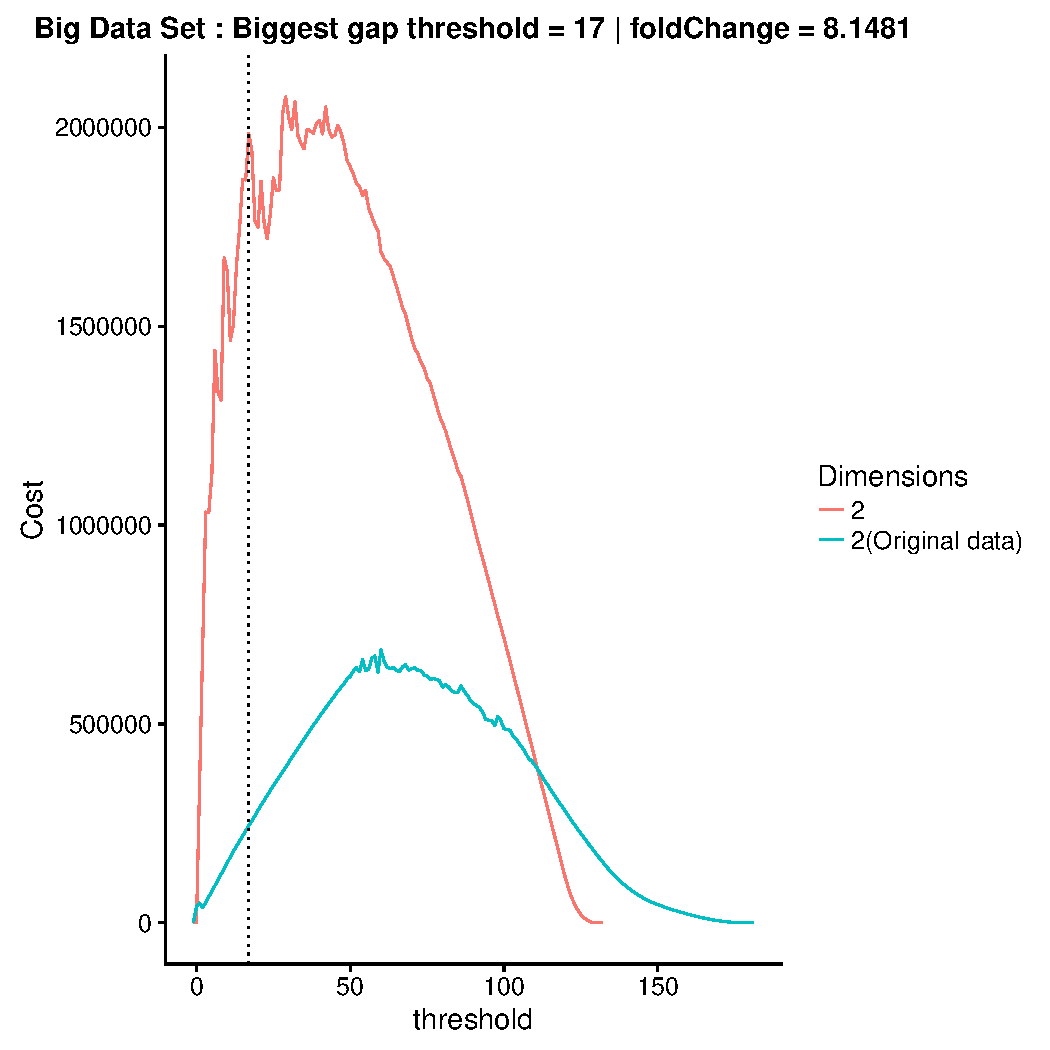
\includegraphics[width=0.9\textwidth]{./plots/plotsCostAndSimAp234/plotBigDataCostAndSim-AP3-S42-K2.pdf}
		\caption{Randomization approach 3: Max gap cost}
		\label{fig:maxGapCostBigDataAp3K2}
	\end{minipage}
\end{figure}

%%%%%%%%%%%%%%%%%%%%%%%%%%%%%%%%%%%%%%%%%%%%%%%%%%
\subsubsection{Randomization Approach 4}
%%%%%%%%%%%%%%%%%%%%%%%%%%%%%%%%%%%%%%%%%%%%%%%%%%
This approach was tested with same number of randomizations and dimensions as approach 3. The max gap was found on dimensions 2, 3, 4, 5 and 10, which each was randomized 4 times. Figure \ref{fig:plotCostsRandomBigDataAp4} shows the distribution of costs across the dimensions, and it looks more promising than approach 3. This is kind of expected as this randomization was made from the exact same similarities as the actual data, in a random ordering. Figures \ref{fig:maxGapCostBigDataAp4K2} and \ref{fig:maxGapCostBigDataAp4K3} shows the most promising results. The thresholds that has the biggest gap are 20 and 15, which is close the the optimum of 17. Noticing the dimensions are 2 and 3. These trials has the opposite statistics as approach 3. Approach 3 had 16/20 where the gap was found at the peak of cost, and 4/20 the gap was found away from the peak. With approach 4 we have 16/20 where the biggest gap is found away from the peak, and 4/20 where the gap is directly on the peak of cost. Although we do not hit the exact same threshold, 17, which had the overall best clustering quality, this approach seems promising.

\begin{figure}[H]
	\centering
	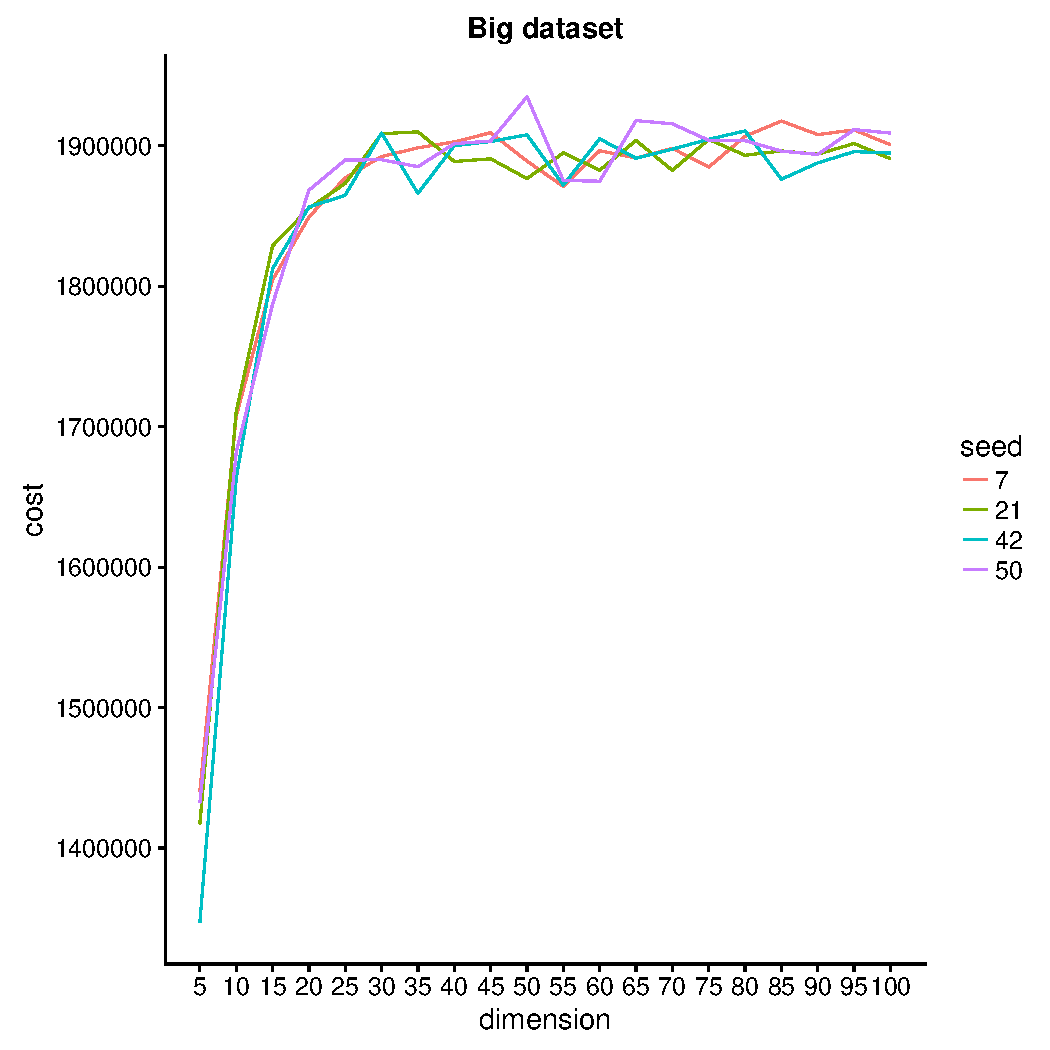
\includegraphics[width=0.80\textwidth]{./plots/plotMaxCostRandomBig/plotCostsRandomBigData-Ap4.pdf}
	\caption{Randomization approach 4: Max cost distribution across dimensions}
	\label{fig:plotCostsRandomBigDataAp4}
\end{figure}


\begin{figure}[H]
	\centering
	\begin{minipage}{0.75\textwidth}
		\centering
		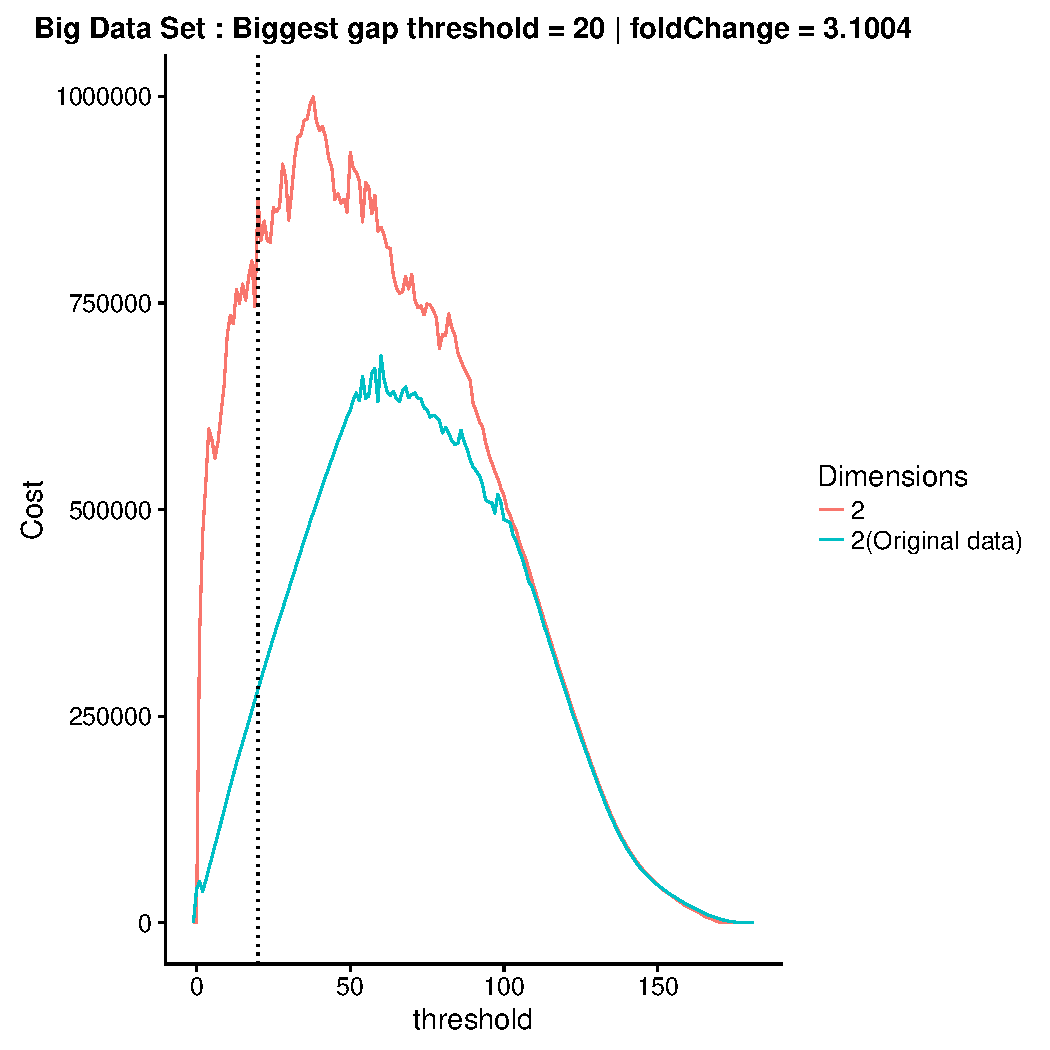
\includegraphics[width=0.9\textwidth]{./plots/plotsCostAndSimAp234/plotBigDataCostAndSim-AP4-S21-K2.pdf}
		\caption{Randomization approach 4: Max gap cost}
		\label{fig:maxGapCostBigDataAp4K2}
	\end{minipage}
	\begin{minipage}{0.75\textwidth}
		\centering
		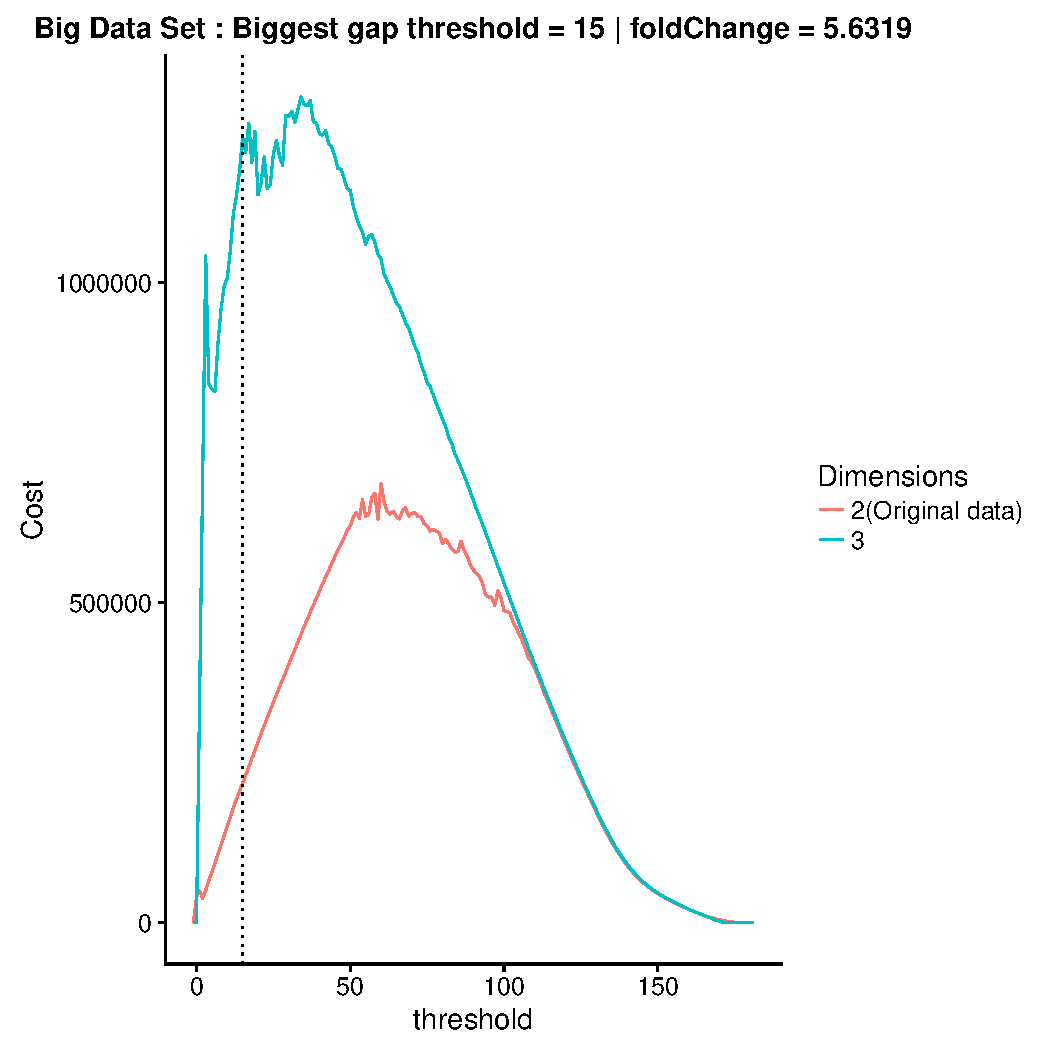
\includegraphics[width=0.9\textwidth]{./plots/plotsCostAndSimAp234/plotBigDataCostAndSim-AP4-S7-K3.pdf}
		\caption{Randomization approach 4: Max gap cost}
		\label{fig:maxGapCostBigDataAp4K3}
	\end{minipage}
\end{figure}

From the 4 tested randomization approaches both 3 and 4 looks promising. Approach 3 has a result which hits the exact same threshold as the optimal clustering result with threshold 17. Approach 4 comes close to this threshold. The closest for approach 4 was threshold 15 and 20. One thing to notice is the number of dimensions on these results which was 2 and 3. At this point it is difficult to say which approach is better than the other. Approach 3 and 4 was each tested 4 times with 5 different dimensions, which is a small sample size. It requires a bigger sample size in order to determine consistency and properly compare the randomization approaches. Considering the statistics for the given trials where the peak was away from the peaking cost, approach 4 seems to be the more promising. Approach 3 and 4 are viewed as feasible randomization. Approach 1 and 2 are not considered as feasible randomizations at this point.
\\

%%%%%%%%%%%%%%%%%%%%%%%%%%%%%%%%%%%%%%%%%%%%%%%%%%
\subsubsection{Randomization and Transitivity-Hierarchical Clustering}
%%%%%%%%%%%%%%%%%%%%%%%%%%%%%%%%%%%%%%%%%%%%%%%%%%
As both approach 3 and 4 looks promising at this point, these are used to assess the max gap cost during the hierarchical clustering. Looking at the max gap cost at each node in the dendrogram should somehow reveal if the split will increase of decrease the quality of the clustering. If the indication is that the quality will decrease if the given node is split, the branch should be cut and returning this node as a cluster in the clustering result. Let $n_{i,j}$ be node i at height j in the dendrogram. If the returned clustering cost from TC is higher than the randomized version of the same node, it indicates the actual node has a worse structure than the randomized. The structure of the randomized node is worse than the actual node, if the cost of the randomized is higher. How to interpret this in terms of a dynamic tree-cutting approach and finding a pattern in which the cuts can be read is unknown at this point. 
Approach 3 and 4 was each tested 9 times on the small dataset, and 9 times on the big dataset. The tests includes both binary search and non-binary search of the hierarchical clustering. The non-binary search was tested 3 times with step as 1 and 3. The binary search test was tested with step 30, and range of allowed splits was 2-10. The same parameters was used on the big dataset. On the following plots the cost axis is made with logarithmic scale as the variables (lines) are scaled differently. The cost at a certain threshold does not necessarily only involve a single cluster/node. If three different nodes are clustered at, e.g., threshold 10, the clustering costs is the sum of costs for all three nodes. Remind that for each node the cost of the randomized will be found as well. Meaning the difference in cost at a given threshold is the difference between the clustering cost of the three nodes and the clustering cost of the three randomized nodes.
On the following plots the difference is scaled into 4 different variables. 'actual' is the direct cost value difference, as as the absolute value. 'avg' is the total difference averaged over the number of involved proteins. 'avgPairs' is the difference over the amount of pairs for the involved proteins. 'foldChange' is the fold change between the actual cost and the randomized cost. As the plots are using logarithmic scale it was not possible to show negative values, thus taking the absolute value. The conversions from a negative to positive fold change is indicated by black points. If the fold change was negative then the randomized data had a clustering cost lower than the actual clustering cost. Often one of the clustering costs are 0, which would set the fold change to $\infty$, where the fold change is manually set to 0.001.

Finding the difference in cost for each node in the dendrogram, THC was tested with the settings in Table \ref{table:testGapTHC}.
\begin{table}[]
	\centering
	\scalebox{0.9}{
		\begin{tabular}{|l|l|l|l|l|l|}
			\hline
			Rand. approach & Dimensions & Seed & Steps & Binary Search & Allowed splits \\\hline
			3 & 5 & 7, 21, 42 & 1, 5 & No  & - \\\hline
			3 & 5 & 7, 21, 42 & 30   & Yes & 2-10 \\\hline
			4 & 5 & 7, 21, 42 & 1, 5 & No  & - \\\hline
			4 & 5 & 7, 21, 42 & 30   & Yes & 2-10 \\\hline
		\end{tabular}
	}
	\caption{Settings for finding the biggest cap at each node in the dendrogram with THC and randomizations. The randomizations scaled the data up to 5 dimensions. Each seed counts as a randomization of the data, $2 \cdot 3$ randomizations for each approach on the given data. This was done on both the small dataset and the big dataset. Steps is the incrementation of threshold for every iteration. Binary Search states if the test was run with binary search on the threshold, until number of splits are in the range of allowed splits.}
	\label{table:testGapTHC}
\end{table}


Figures \ref{fig:hcMaxGapSmallDataAp3Step1NoBinary} through \ref{fig:hcMaxGapBigDataAp3Step30Binary} shows the difference in cost for approach 3 and 4 for the small and big dataset. What to interpret from these plots, or even if they show any valuable information at all is the next step in the project. One way to improve the plots would be taking the average for each approach, where these plots are for a single run. Due to the scope of the project it was not possible to gain any further knowledge. It is needed to analyze the plots, deriving any patterns indicating a cut. Altering the hierarchical clustering algorithm making it possible to make the cuts on branches, and returning the resulting clustering. To determine the quality the F-measure is calculated and the clustering can be validated. The procedure of analyzing the plots and finding any valuable patterns, or information, in terms of the cost difference is the on going process. With the proper information or pattern the dynamic cut of the tree can be derived returning the optimal clustering. If there is no valuable information to gain from the plots, another approach to analyzing the difference in cost needs to be considered, or maybe another randomization approach. Thus the next steps in the project would be:
\begin{itemize}
	\item Analyze the plots for the difference in cost at each node in the dendrogram. Goal is to find a pattern or anything that indicates where to cut the branches in the dendrograms, in order to obtain a tree which is dynamically cut on different levels. The resulting tree is the optimal clustering.
	\item Alter the algorithm for THC, such that we can cut the branches at different levels. Depending on the difference in costs it makes a decision for the cut of branches, and a clustering can be returned.
	\item The clustering result from THC will be compared to the gold standard to gain a quality measure of the clustering.
	\item Analyzing the plots and try different approaches on where to cut is trial-and-error. This step goes on until we find this approach to parameterless clustering by dynamic tree-cutting either feasible or infeasible.
\end{itemize}

\begin{figure}[H]
	\centering
	\begin{minipage}{0.80\textwidth}
		\centering
		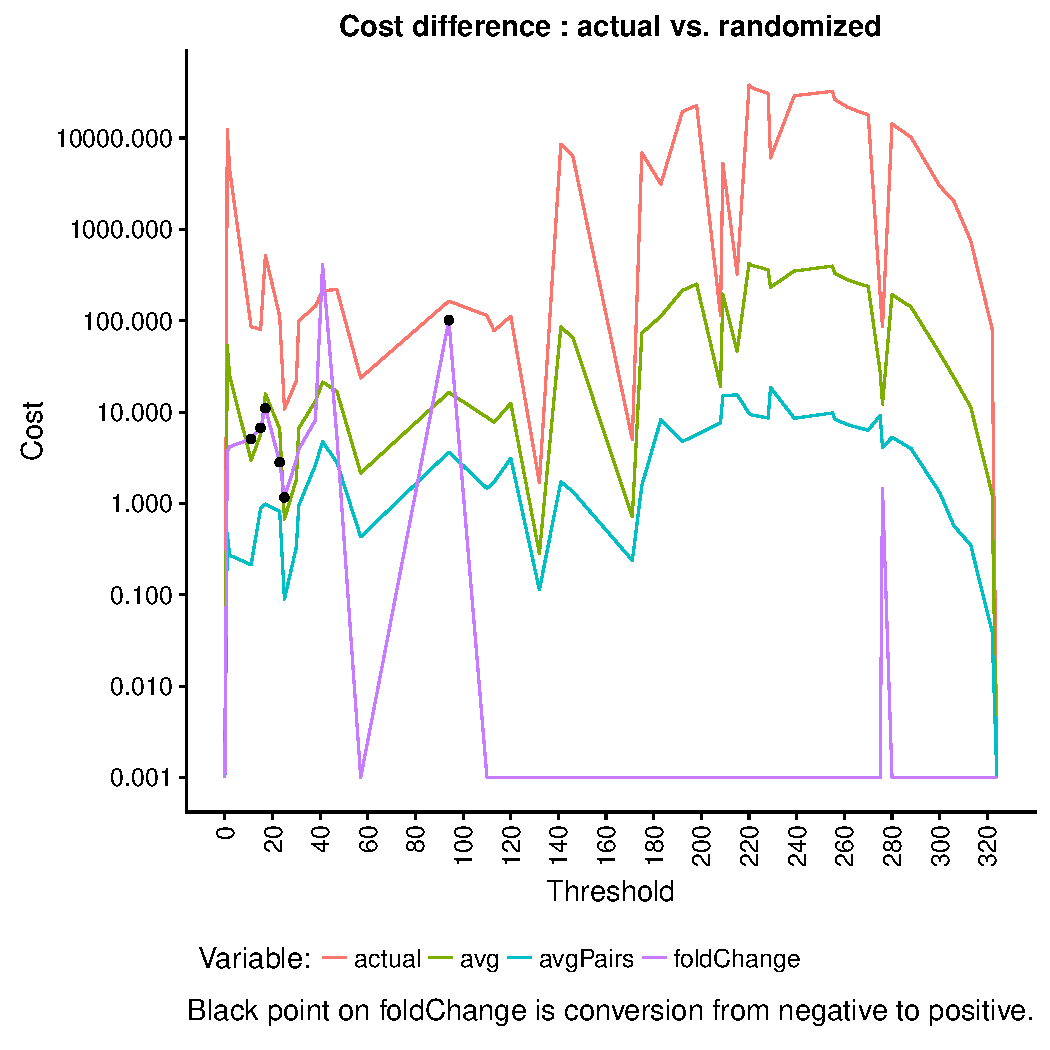
\includegraphics[width=0.9\textwidth]{./plots/plotCostGap/plotCostGapSmallDataAp3Step1K5Seed21NoBinary.pdf}
		\caption{Small data, approach 3, step = 1, non-binary search}
		\label{fig:hcMaxGapSmallDataAp3Step1NoBinary}
	\end{minipage}
	\begin{minipage}{0.80\textwidth}
		\centering
		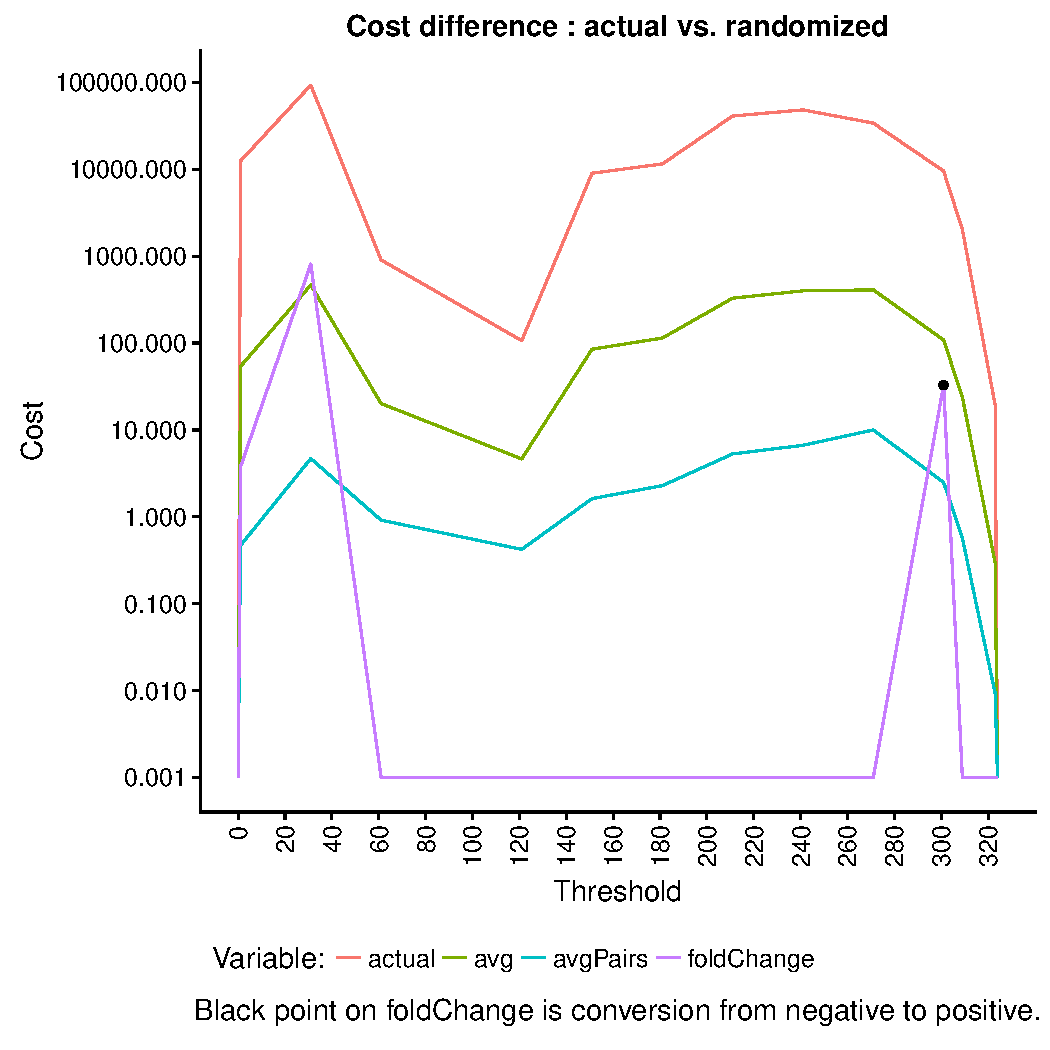
\includegraphics[width=0.9\textwidth]{./plots/plotCostGap/plotCostGapSmallDataAp3Step30K5Seed7Binary.pdf}
		\caption{Small data, approach 3, step = 30, binary search, allowed range of splits 2-10}
		\label{fig:hcMaxGapSmallDataAp3Step30Binary}
	\end{minipage}
\end{figure}

\begin{figure}[H]
	\centering
	\begin{minipage}{0.80\textwidth}
		\centering
		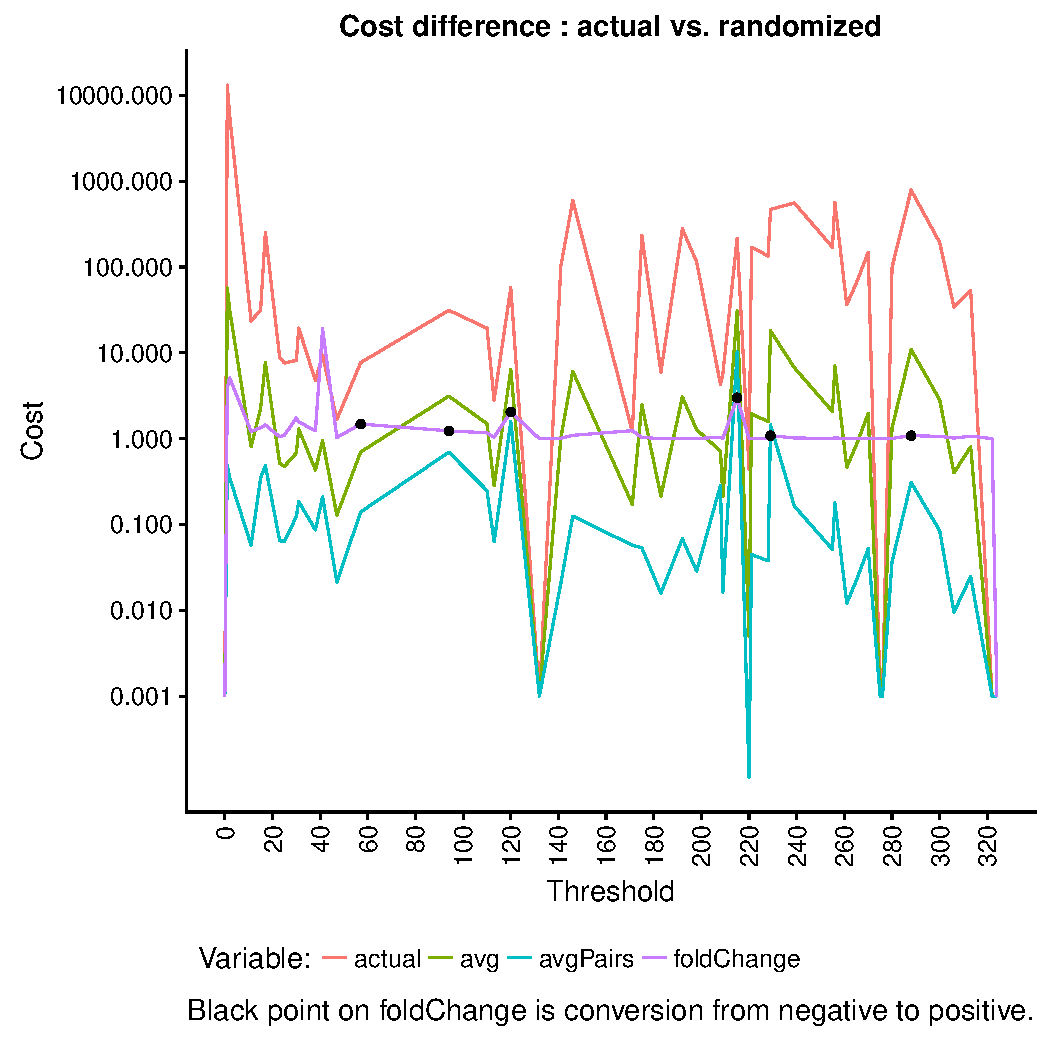
\includegraphics[width=0.9\textwidth]{./plots/plotCostGap/plotCostGapSmallDataAp4Step1K5Seed7NoBinary.pdf}
		\caption{Small data, approach 4, step = 1, non-binary search}
		\label{fig:hcMaxGapSmallDataAp4Step1NoBinary}
	\end{minipage}
	\begin{minipage}{0.80\textwidth}
		\centering
		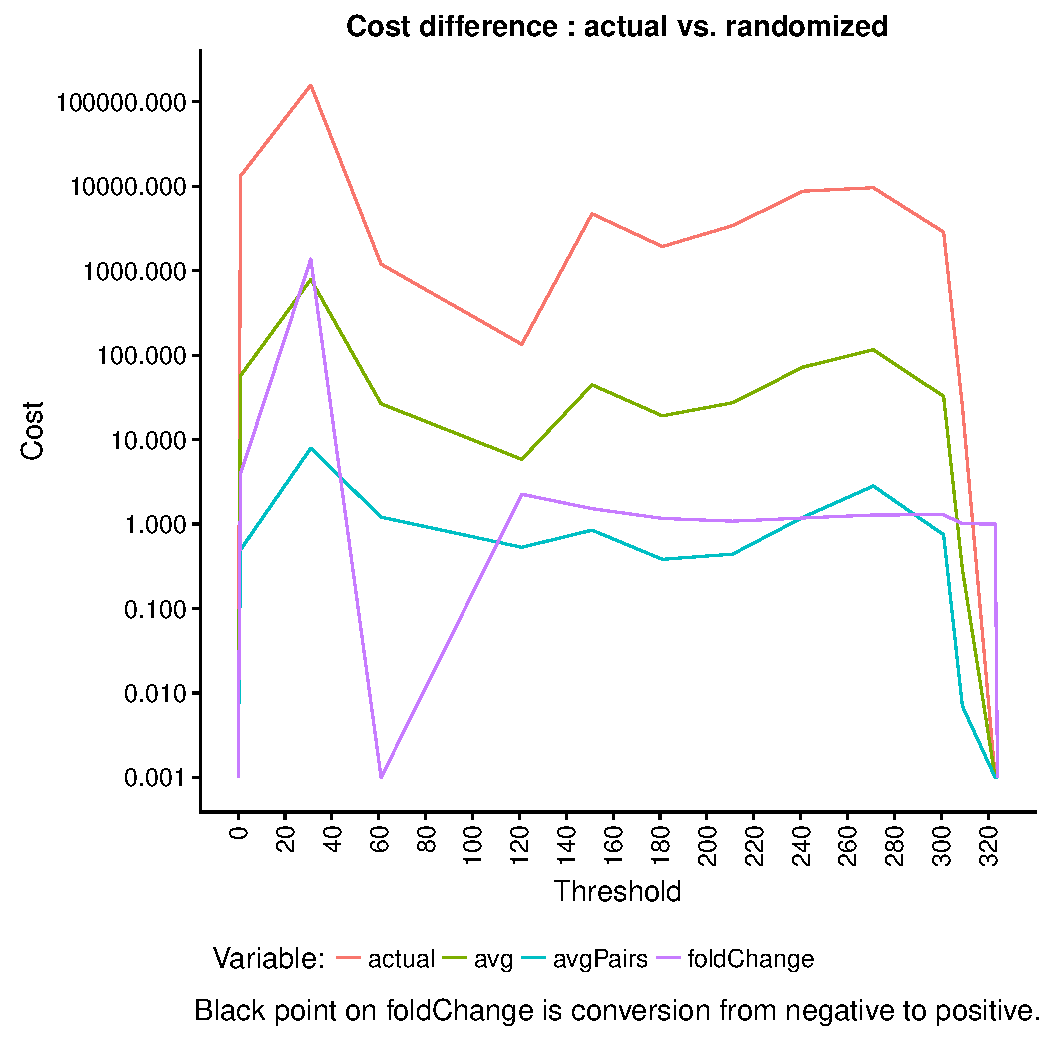
\includegraphics[width=0.9\textwidth]{./plots/plotCostGap/plotCostGapSmallDataAp4Step30K5Seed42Binary.pdf}
		\caption{Small data, approach 4, step = 30, binary search, allowed range of splits 2-10}
		\label{fig:hcMaxGapSmallDataAp4Step30Binary}
	\end{minipage}
\end{figure}

\begin{figure}[H]
	\centering
	\begin{minipage}{0.80\textwidth}
		\centering
		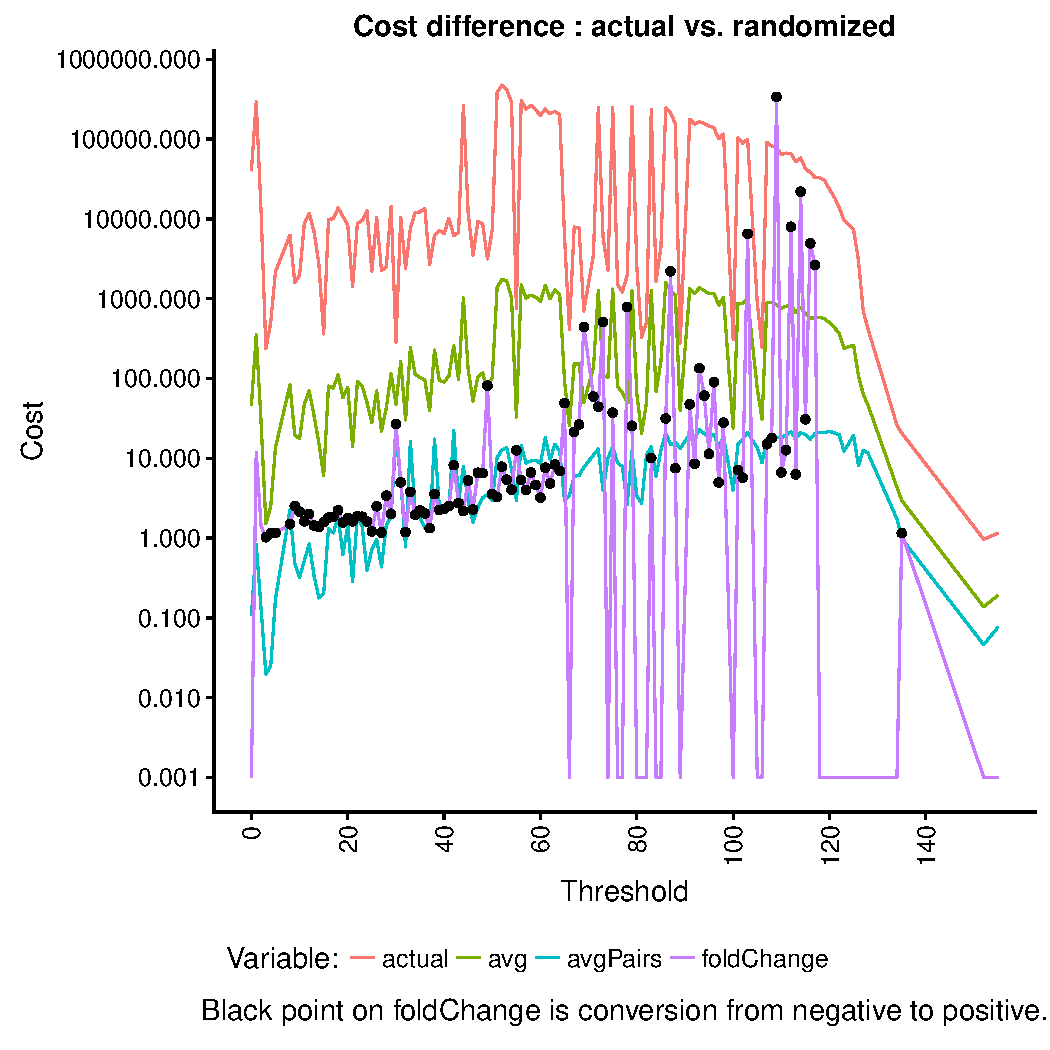
\includegraphics[width=0.9\textwidth]{./plots/plotCostGap/plotCostGapBigDataAp3Step1K5Seed42NoBinary.pdf}
		\caption{Big data, approach 3, step = 1, non-binary search}
		\label{fig:hcMaxGapBigDataAp3Step1NoBinary}
	\end{minipage}
	\begin{minipage}{0.80\textwidth}
		\centering
		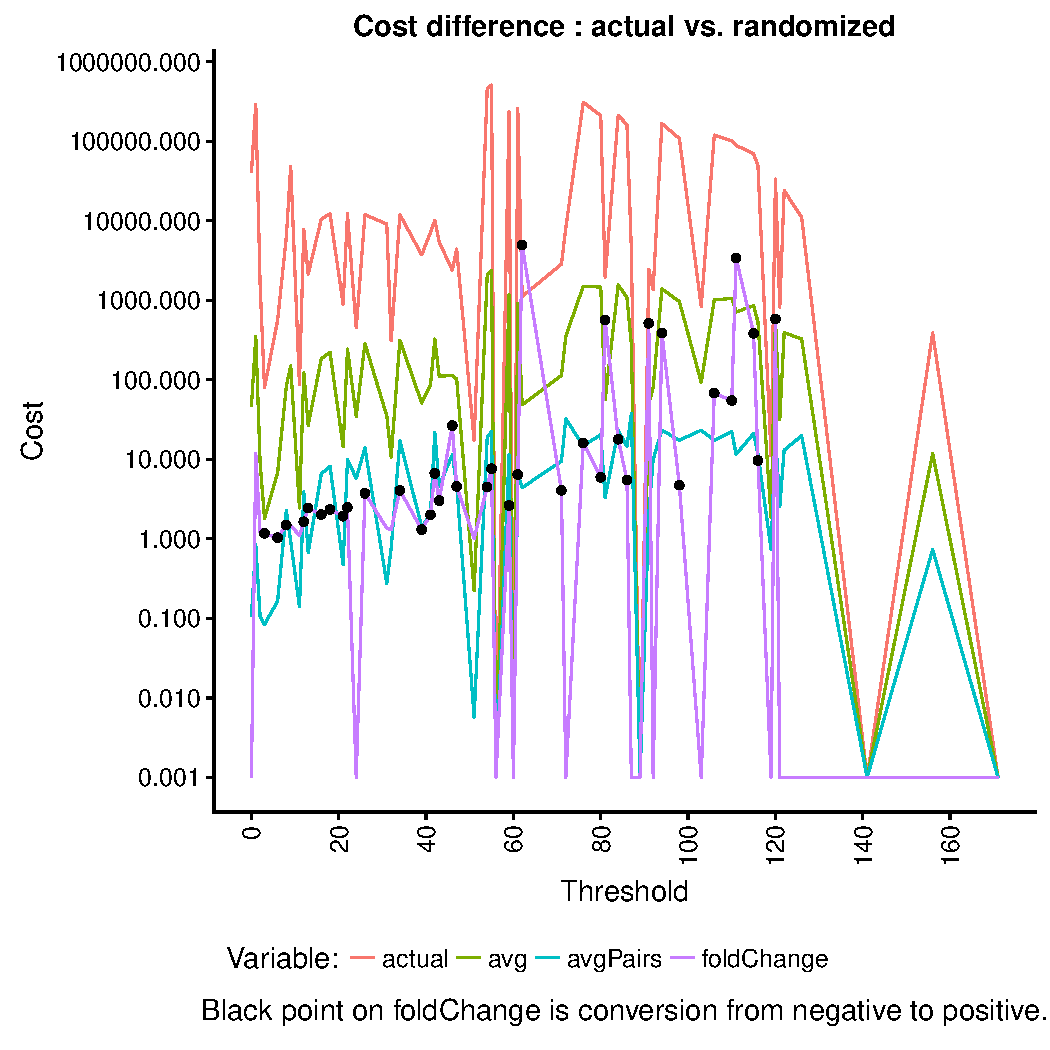
\includegraphics[width=0.9\textwidth]{./plots/plotCostGap/plotCostGapBigDataAp3Step30K5Seed7Binary.pdf}
		\caption{Big data, approach 3, step = 30, binary search, allowed range of splits 2-10}
		\label{fig:hcMaxGapBigDataAp3Step30Binary}
	\end{minipage}
\end{figure}

\begin{figure}[H]
	\centering
	\begin{minipage}{0.80\textwidth}
		\centering
		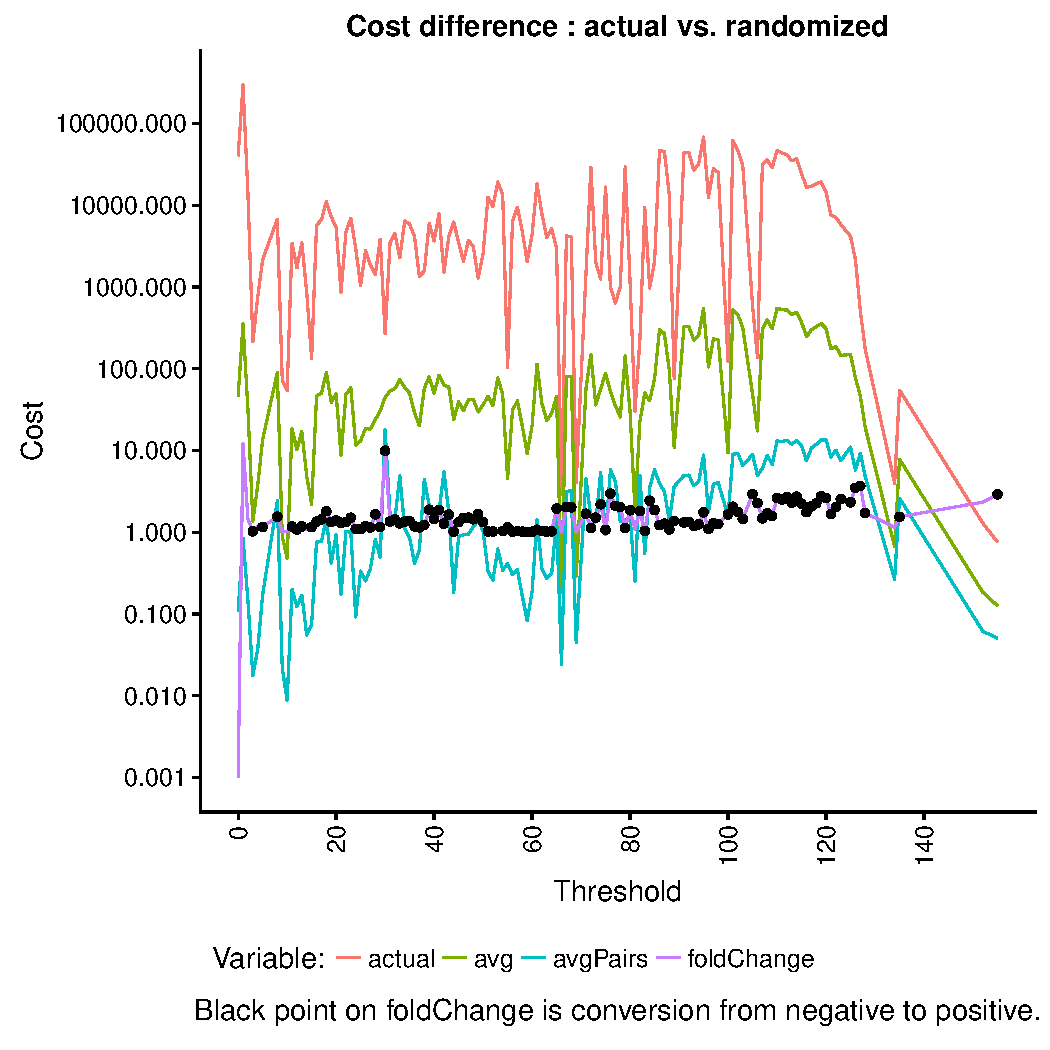
\includegraphics[width=0.9\textwidth]{./plots/plotCostGap/plotCostGapBigDataAp4Step1K5Seed42NoBinary.pdf}
		\caption{Big data, approach 4, step = 1, non-binary search}
		\label{fig:hcMaxGapBigDataAp4Step1NoBinary}
	\end{minipage}
	\begin{minipage}{0.80\textwidth}
		\centering
		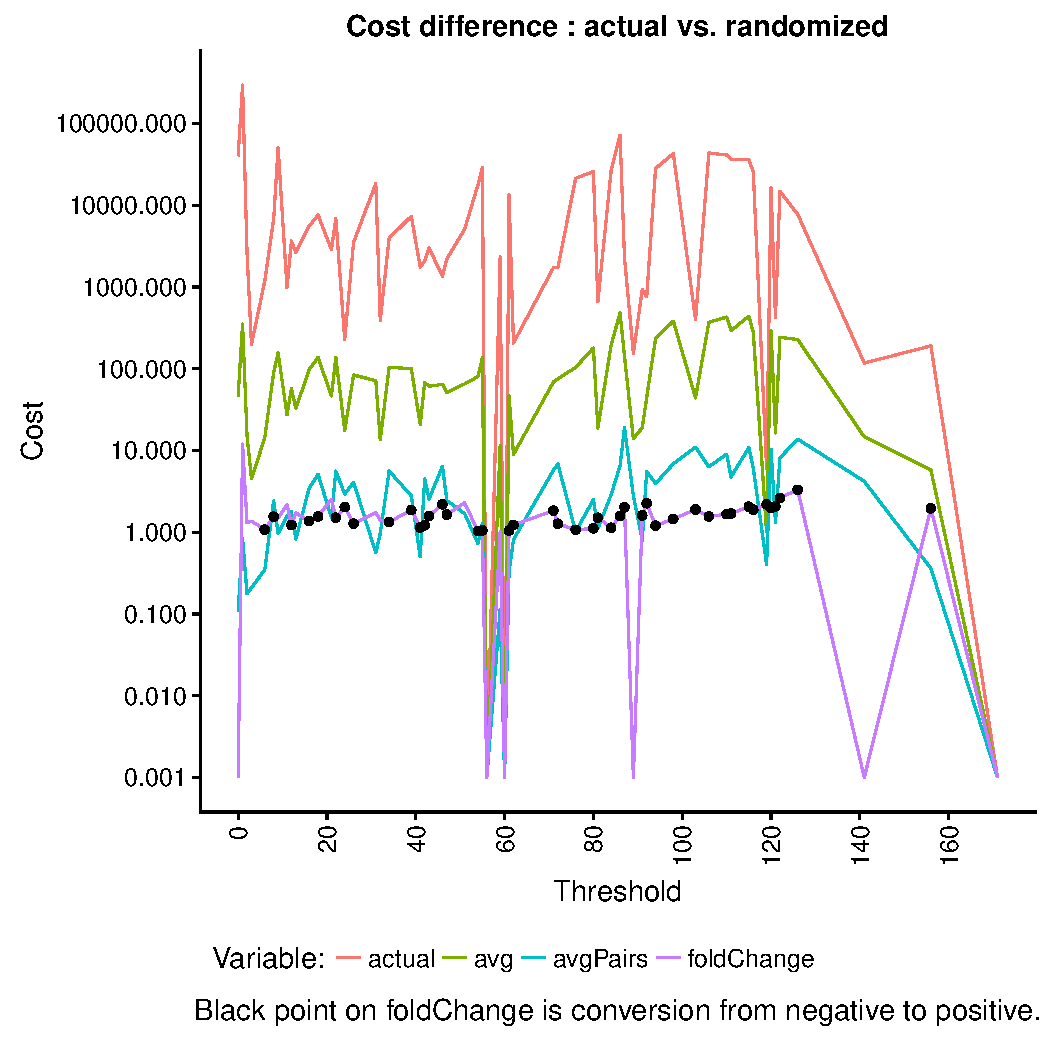
\includegraphics[width=0.9\textwidth]{./plots/plotCostGap/plotCostGapBigDataAp4Step30K5Seed42Binary.pdf}
		\caption{Big data, approach 4, step = 30, binary search, allowed range of splits 2-10}
		\label{fig:hcMaxGapBigDataAp4Step30Binary}
	\end{minipage}
\end{figure}

%%%%%%%%%%%%%%%%%%%%%%%%%%%%%%%%%%%%%%%%%%%%%%%%%%
%%%%%%%%%%%%%%%%%%%%%%%%%%%%%%%%%%%%%%%%%%%%%%%%%%
%%%%%%%%%%%%%%%%%%%%%%%%%%%%%%%%%%%%%%%%%%%%%%%%%%
\newpage
\section{Implementation}
%%%%%%%%%%%%%%%%%%%%%%%%%%%%%%%%%%%%%%%%%%%%%%%%%%
%%%%%%%%%%%%%%%%%%%%%%%%%%%%%%%%%%%%%%%%%%%%%%%%%%
%%%%%%%%%%%%%%%%%%%%%%%%%%%%%%%%%%%%%%%%%%%%%%%%%%
R was the chosen language for the project as it eases the work around matrices, also has rather easy customization for producing plots. RStudio was the used IDE. R has a lot of built-in methods which eased the coding process, as not everything had to be invented from scratch. Also, it is possible to install different package for the suiting of your needs. Transitivity Clustering was given as an R package. Hierarchical Clustering is already implemented in R, meaning that we could use the plotting features for the dendrograms. From the package MASS we used the isoMDS() method for the multidimensional scaling. From the package 'stats' the method cmdscale() was used in correlation with isoMDS(). All coding and testing has been done on a Linux Mint environment, with Intel Core I7 and 32GB of RAM.
All code and various testing output and plots can be viewed at: https://github.com/simkn15/Parameterless-clustering-by-dynamic-tree-cutting

%%%%%%%%%%%%%%%%%%%%%%%%%%%%%%%%%%%%%%%%%%%%%%%%%%
%%%%%%%%%%%%%%%%%%%%%%%%%%%%%%%%%%%%%%%%%%%%%%%%%%
%%%%%%%%%%%%%%%%%%%%%%%%%%%%%%%%%%%%%%%%%%%%%%%%%%
\newpage
\section{Conclusion}
%%%%%%%%%%%%%%%%%%%%%%%%%%%%%%%%%%%%%%%%%%%%%%%%%%
%%%%%%%%%%%%%%%%%%%%%%%%%%%%%%%%%%%%%%%%%%%%%%%%%%
%%%%%%%%%%%%%%%%%%%%%%%%%%%%%%%%%%%%%%%%%%%%%%%%%%
We wanted to investigate parameterless clustering by dynamic-tree cutting. The first step was to extend Transitivity Clustering(TC) into Hierarchical Clustering(HC), we call this Transitivity-Hierarchical Clustering(THC). In order to evaluate a clustering according to to the gold standard of the dataset, the Brown dataset, F-measure was the implemented quality measure. The implementation of F-measure is feasible as we get close to the same results as \cite{clustEval} in terms of the threshold for the optimal clustering for the small dataset. In our case the optimal threshold was 47 with F-measure of 0.981 where \cite{clustEval} found threshold 48.86 with F-measure 0.986. Comparing the dendrograms of THC and the standard implementation og hierarchical clustering in R, the implementation is working as intended and produces a valid dendrogram. For each node in the dendrogram we look at the clustering cost of the actual data and a randomized version of the same node. The difference in cost should indicate where to cut each branch in the tree. The resulting tree is therefore cut on different levels, and is the optimal clustering. Multiple randomization approaches was tested in order to randomize each node in the dendrogram. In total of 4 different approaches was tested. TC returned costs that were too high on the first approach, above 1,000,000, for the small dataset. The actual costs peak at around 60,000. This is due to no structure in the randomized dataset. Each approach step by step gets a more structural randomization, which looks to be feasible with randomization approach 3 and 4. Approach 1 and 2 was determined as infeasible. Multiple tests was run with THC to find the difference in costs in all nodes in the dendrogram. However, unexpectedly, we did not get to analyze the plots from these tests, because of the scope of the project. Further steps must be taken in order to validate our approach for parameterless clustering by dynamic tree-cutting. (1) Analyze the plots of cost differences for all nodes in the dendrogram. (2) Alter the THC algorithm such that it can the branches in the dendrogram on different levels, and return a clustering result. (3) COmpare the clustering result to the gold standard with F-measure. (4) Repeat the steps of analyzing and change the approach of when to cut a branch, until we find this approach to parameterless clustering by dynamic tree-cutting either feasible or infeasible.


\newpage
\bibliographystyle{abbrv}
\bibliography{references}



\end{document}
